%*************************************************************************
% A Classic Thesis Style
% An Homage to The Elements of Typographic Style
%
% Copyright (C) 2017 André Miede and Ivo Pletikosić
%
% If you like the style then I would appreciate a postcard. My address
% can be found in the file ClassicThesis.pdf. A collection of the
% postcards I received so far is available online at
% http://postcards.miede.de
%
% License:
% This program is free software; you can redistribute it and/or modify
% it under the terms of the GNU General Public License as published by
% the Free Software Foundation; either version 2 of the License, or
% (at your option) any later version.
%
% This program is distributed in the hope that it will be useful,
% but WITHOUT ANY WARRANTY; without even the implied warranty of
% MERCHANTABILITY or FITNESS FOR A PARTICULAR PURPOSE.  See the
% GNU General Public License for more details.
%
% You should have received a copy of the GNU General Public License
% along with this program; see the file COPYING.  If not, write to
% the Free Software Foundation, Inc., 59 Temple Place - Suite 330,
% Boston, MA 02111-1307, USA.
%
% PLEASE SEE ALSO THE AUTHORS' NOTE REGARDING THIS LICENSE
% IN THE DOCUMENTATION (ClassicThesis.pdf --> Chapter 1 / Chapter01.tex)
%*************************************************************************
\RequirePackage{silence} % :-\
    \WarningFilter{scrreprt}{Usage of package `titlesec'}
    %\WarningFilter{scrreprt}{Activating an ugly workaround}
    \WarningFilter{titlesec}{Non standard sectioning command detected}
\documentclass[ openright,titlepage,numbers=noenddot,headinclude,%twoside, %1headlines,% letterpaper a4paper
                footinclude=true,cleardoublepage=empty,abstractoff, % <--- obsolete, remove (todo)
                BCOR=5mm,paper=a4,fontsize=11pt,%11pt,a4paper,%
                ngerman,american,%lockflag%
                ]{scrreprt}

%*************************************************************************
% Note: Make all your adjustments in here
%*************************************************************************
% ****************************************************************************************************
% hdathesis-config.tex 
% Use it at the beginning of your thesis.tex, or as a LaTeX Preamble 
% in your thesis.{tex,lyx} with % ****************************************************************************************************
% hdathesis-config.tex 
% Use it at the beginning of your thesis.tex, or as a LaTeX Preamble 
% in your thesis.{tex,lyx} with % ****************************************************************************************************
% hdathesis-config.tex 
% Use it at the beginning of your thesis.tex, or as a LaTeX Preamble 
% in your thesis.{tex,lyx} with \input{hdathesis-config}
% ****************************************************************************************************

% ****************************************************************************************************
% 1. Personal data and user ad-hoc commands
% ****************************************************************************************************
\newcommand{\myTitle}{Entwicklung eines Chat SaaS mit Kubernetes in Gaia-X kompatibler Cloud\xspace}
%\newcommand{\mySubtitle}{An Homage to The Elements of Typographic Style\xspace}
\newcommand{\myDegree}{Bachelor of Science (B.Sc.)\xspace} 
\newcommand{\myName}{Lukas Höhl\xspace}
\newcommand{\myId}{761527\xspace}
\newcommand{\myProf}{Prof. Dr. Peter Altenbernd\xspace}
\newcommand{\myOtherProf}{Prof. Arnim Malcherek\xspace}
\newcommand{\myFaculty}{Fachbereich Informatik\xspace}
\newcommand{\myUni}{Hochschule Darmstadt\xspace}
\newcommand{\myLocation}{Darmstadt\xspace}
\newcommand{\myTime}{3. Februar 2022\xspace}
\newcommand{\myVersion}{version 1.0\xspace}

% ****************************************************************************************************
% 2. Is it a master thesis?
% ****************************************************************************************************
%\PassOptionsToPackage{master}{hdahesis} % uncomment if this is a master thesis 

% ****************************************************************************************************
% 3. Does the thesis have a lock flag?
% ****************************************************************************************************
%\PassOptionsToPackage{lockflag}{hdathesis} % uncomment if this thesis has a lock flag 

% ****************************************************************************************************
% 4. Loading some handy packages
% ****************************************************************************************************
% ****************************************************************************************************
% Packages with options that might require adjustments
% ****************************************************************************************************

%\PassOptionsToPackage{ngerman,american}{babel}   % change this to your language(s)
% Spanish languages need extra options in order to work with this template
%\PassOptionsToPackage{spanish,es-lcroman}{babel}
\usepackage{babel}



% ****************************************************************************************************

% ****************************************************************************************************
% 1. Personal data and user ad-hoc commands
% ****************************************************************************************************
\newcommand{\myTitle}{Entwicklung eines Chat SaaS mit Kubernetes in Gaia-X kompatibler Cloud\xspace}
%\newcommand{\mySubtitle}{An Homage to The Elements of Typographic Style\xspace}
\newcommand{\myDegree}{Bachelor of Science (B.Sc.)\xspace} 
\newcommand{\myName}{Lukas Höhl\xspace}
\newcommand{\myId}{761527\xspace}
\newcommand{\myProf}{Prof. Dr. Peter Altenbernd\xspace}
\newcommand{\myOtherProf}{Prof. Arnim Malcherek\xspace}
\newcommand{\myFaculty}{Fachbereich Informatik\xspace}
\newcommand{\myUni}{Hochschule Darmstadt\xspace}
\newcommand{\myLocation}{Darmstadt\xspace}
\newcommand{\myTime}{3. Februar 2022\xspace}
\newcommand{\myVersion}{version 1.0\xspace}

% ****************************************************************************************************
% 2. Is it a master thesis?
% ****************************************************************************************************
%\PassOptionsToPackage{master}{hdahesis} % uncomment if this is a master thesis 

% ****************************************************************************************************
% 3. Does the thesis have a lock flag?
% ****************************************************************************************************
%\PassOptionsToPackage{lockflag}{hdathesis} % uncomment if this thesis has a lock flag 

% ****************************************************************************************************
% 4. Loading some handy packages
% ****************************************************************************************************
% ****************************************************************************************************
% Packages with options that might require adjustments
% ****************************************************************************************************

%\PassOptionsToPackage{ngerman,american}{babel}   % change this to your language(s)
% Spanish languages need extra options in order to work with this template
%\PassOptionsToPackage{spanish,es-lcroman}{babel}
\usepackage{babel}



% ****************************************************************************************************

% ****************************************************************************************************
% 1. Personal data and user ad-hoc commands
% ****************************************************************************************************
\newcommand{\myTitle}{Entwicklung eines Chat SaaS mit Kubernetes in Gaia-X kompatibler Cloud\xspace}
%\newcommand{\mySubtitle}{An Homage to The Elements of Typographic Style\xspace}
\newcommand{\myDegree}{Bachelor of Science (B.Sc.)\xspace} 
\newcommand{\myName}{Lukas Höhl\xspace}
\newcommand{\myId}{761527\xspace}
\newcommand{\myProf}{Prof. Dr. Peter Altenbernd\xspace}
\newcommand{\myOtherProf}{Prof. Arnim Malcherek\xspace}
\newcommand{\myFaculty}{Fachbereich Informatik\xspace}
\newcommand{\myUni}{Hochschule Darmstadt\xspace}
\newcommand{\myLocation}{Darmstadt\xspace}
\newcommand{\myTime}{3. Februar 2022\xspace}
\newcommand{\myVersion}{version 1.0\xspace}

% ****************************************************************************************************
% 2. Is it a master thesis?
% ****************************************************************************************************
%\PassOptionsToPackage{master}{hdahesis} % uncomment if this is a master thesis 

% ****************************************************************************************************
% 3. Does the thesis have a lock flag?
% ****************************************************************************************************
%\PassOptionsToPackage{lockflag}{hdathesis} % uncomment if this thesis has a lock flag 

% ****************************************************************************************************
% 4. Loading some handy packages
% ****************************************************************************************************
% ****************************************************************************************************
% Packages with options that might require adjustments
% ****************************************************************************************************

%\PassOptionsToPackage{ngerman,american}{babel}   % change this to your language(s)
% Spanish languages need extra options in order to work with this template
%\PassOptionsToPackage{spanish,es-lcroman}{babel}
\usepackage{babel}



% ****************************************************************************************************
% classicthesis-config.tex
% formerly known as loadpackages.sty, classicthesis-ldpkg.sty, and classicthesis-preamble.sty
% Use it at the beginning of your ClassicThesis.tex, or as a LaTeX Preamble
% in your ClassicThesis.{tex,lyx} with % ****************************************************************************************************
% classicthesis-config.tex
% formerly known as loadpackages.sty, classicthesis-ldpkg.sty, and classicthesis-preamble.sty
% Use it at the beginning of your ClassicThesis.tex, or as a LaTeX Preamble
% in your ClassicThesis.{tex,lyx} with % ****************************************************************************************************
% classicthesis-config.tex
% formerly known as loadpackages.sty, classicthesis-ldpkg.sty, and classicthesis-preamble.sty
% Use it at the beginning of your ClassicThesis.tex, or as a LaTeX Preamble
% in your ClassicThesis.{tex,lyx} with \input{classicthesis-config}
% ****************************************************************************************************
% If you like the classicthesis, then I would appreciate a postcard.
% My address can be found in the file ClassicThesis.pdf. A collection
% of the postcards I received so far is available online at
% http://postcards.miede.de
% ****************************************************************************************************


% ****************************************************************************************************
% 0. Set the encoding of your files. UTF-8 is the only sensible encoding nowadays. If you can't read
% äöüßáéçèê∂åëæƒÏ€ then change the encoding setting in your editor, not the line below. If your editor
% does not support utf8 use another editor!
% ****************************************************************************************************
\PassOptionsToPackage{utf8}{inputenc}
  \usepackage{inputenc}

% ****************************************************************************************************
% 1. Configure classicthesis for your needs here, e.g., remove "drafting" below
% in order to deactivate the time-stamp on the pages
% (see ClassicThesis.pdf for more information):
% ****************************************************************************************************
\PassOptionsToPackage{
  drafting=false,   % print version information on the bottom of the pages
  tocaligned=false, % the left column of the toc will be aligned (no indentation)
  dottedtoc=true,   % page numbers in ToC flushed right
  parts=true,       % use part division
  eulerchapternumbers=true, % use AMS Euler for chapter font (otherwise Palatino)
  linedheaders=false,       % chaper headers will have line above and beneath
  floatperchapter=true,     % numbering per chapter for all floats (i.e., Figure 1.1)
  listings=true,    % load listings package and setup LoL
  subfig=true,      % setup for preloaded subfig package
  eulermath=false,  % use awesome Euler fonts for mathematical formulae (only with pdfLaTeX)
  beramono=true,    % toggle a nice monospaced font (w/ bold)
  minionpro=false   % setup for minion pro font; use minion pro small caps as well (only with pdfLaTeX)
}{classicthesis}


% ****************************************************************************************************
% 2. Personal data and user ad-hoc commands
% ****************************************************************************************************
%\newcommand{\myTitle}{A Classic Thesis Style\xspace}
%\newcommand{\mySubtitle}{An Homage to The Elements of Typographic Style\xspace}
%\newcommand{\myDegree}{Doktor-Ingenieur (Dr.-Ing.)\xspace}
%\newcommand{\myName}{André Miede\xspace}
%\newcommand{\myProf}{Put name here\xspace}
%\newcommand{\myOtherProf}{Put name here\xspace}
%\newcommand{\mySupervisor}{Put name here\xspace}
%\newcommand{\myFaculty}{Put data here\xspace}
%\newcommand{\myDepartment}{Put data here\xspace}
%\newcommand{\myUni}{Put data here\xspace}
%\newcommand{\myLocation}{Saarbrücken\xspace}
%\newcommand{\myTime}{October 2017\xspace}
%\newcommand{\myVersion}{version 4.4}

% ********************************************************************
% Setup, finetuning, and useful commands
% ********************************************************************
\newcounter{dummy} % necessary for correct hyperlinks (to index, bib, etc.)
\newlength{\abcd} % for ab..z string length calculation
\providecommand{\mLyX}{L\kern-.1667em\lower.25em\hbox{Y}\kern-.125emX\@}
\newcommand{\ie}{i.\,e.}
\newcommand{\Ie}{I.\,e.}
\newcommand{\eg}{e.\,g.}
\newcommand{\Eg}{E.\,g.}
% ****************************************************************************************************


% ****************************************************************************************************
% 3. Loading some handy packages
% ****************************************************************************************************
% ********************************************************************
% Packages with options that might require adjustments
% ********************************************************************
%\PassOptionsToPackage{ngerman,american}{babel}   % change this to your language(s), main language last
% Spanish languages need extra options in order to work with this template
%\PassOptionsToPackage{spanish,es-lcroman}{babel}
\usepackage{babel}

\usepackage{csquotes}

\PassOptionsToPackage{%
  %backend=biber,bibencoding=utf8, %instead of bibtex
  backend=bibtex8,bibencoding=ascii,%
  language=auto,%
  style=numeric-comp,%
  %style=alphabetic,%
  %style=authoryear-comp, % Author 1999, 2010
  %bibstyle=authoryear,dashed=false, % dashed: substitute rep. author with ---
  sorting=nyt, % name, year, title
  maxbibnames=10, % default: 3, et al.
  %backref=true,%
  natbib=true % natbib compatibility mode (\citep and \citet still work)
}{biblatex}
  \usepackage{biblatex}

\PassOptionsToPackage{fleqn}{amsmath}       % math environments and more by the AMS
  \usepackage{amsmath}

\PassOptionsToPackage{doublespacing}{hdathesis}  % options: abbrev exam big wiwi english master
  \usepackage{hdathesis}

% ********************************************************************
% General useful packages
% ********************************************************************
\PassOptionsToPackage{T1}{fontenc} % T2A for cyrillics
  \usepackage{fontenc}
\usepackage{textcomp} % fix warning with missing font shapes
\usepackage{scrhack} % fix warnings when using KOMA with listings package
\usepackage{xspace} % to get the spacing after macros right
\usepackage{mparhack} % get marginpar right
%\usepackage{fixltx2e} % fixes some LaTeX stuff --> since 2015 in the LaTeX kernel (see below)
% \usepackage[latest]{latexrelease} % emulate newer kernel version if older is detected
\PassOptionsToPackage{printonlyused,smaller}{acronym}
  \usepackage{acronym} % nice macros for handling all acronyms in the thesis
  %\renewcommand{\bflabel}[1]{{#1}\hfill} % fix the list of acronyms --> no longer working
  %\renewcommand*{\acsfont}[1]{\textsc{#1}}
  %\renewcommand*{\aclabelfont}[1]{\acsfont{#1}}
  %\def\bflabel#1{{#1\hfill}}
  \def\bflabel#1{{\acsfont{#1}\hfill}}
  \def\aclabelfont#1{\acsfont{#1}}
% ****************************************************************************************************
%\usepackage{pgfplots} % External TikZ/PGF support (thanks to Andreas Nautsch)
%\usetikzlibrary{external}
%\tikzexternalize[mode=list and make, prefix=ext-tikz/]
% ****************************************************************************************************


% ****************************************************************************************************
% 4. Setup floats: tables, (sub)figures, and captions
% ****************************************************************************************************
\usepackage{tabularx} % better tables
  \setlength{\extrarowheight}{3pt} % increase table row height
\newcommand{\tableheadline}[1]{\multicolumn{1}{c}{\spacedlowsmallcaps{#1}}}
\newcommand{\myfloatalign}{\centering} % to be used with each float for alignment
\usepackage{caption}
% Thanks to cgnieder and Claus Lahiri
% http://tex.stackexchange.com/questions/69349/spacedlowsmallcaps-in-caption-label
% [REMOVED DUE TO OTHER PROBLEMS, SEE ISSUE #82]
%\DeclareCaptionLabelFormat{smallcaps}{\bothIfFirst{#1}{~}\MakeTextLowercase{\textsc{#2}}}
%\captionsetup{font=small,labelformat=smallcaps} % format=hang,
\captionsetup{font=small} % format=hang,
\usepackage{subfig}
% ****************************************************************************************************


% ****************************************************************************************************
% 5. Setup code listings
% ****************************************************************************************************
\usepackage{listings}
%\lstset{emph={trueIndex,root},emphstyle=\color{BlueViolet}}%\underbar} % for special keywords
\lstset{language=[LaTeX]Tex,%C++,
  morekeywords={PassOptionsToPackage,selectlanguage},
  keywordstyle=\color{RoyalBlue},%\bfseries,
  basicstyle=\small\ttfamily,
  %identifierstyle=\color{NavyBlue},
  commentstyle=\color{Green}\ttfamily,
  stringstyle=\rmfamily,
  numbers=none,%left,%
  numberstyle=\scriptsize,%\tiny
  stepnumber=5,
  numbersep=8pt,
  showstringspaces=false,
  breaklines=true,
  %frameround=ftff,
  %frame=single,
  belowcaptionskip=.75\baselineskip
  %frame=L
}
% ****************************************************************************************************


% ****************************************************************************************************
% 6. PDFLaTeX, hyperreferences, and citation backreferences
% ****************************************************************************************************
% ********************************************************************
% Using PDFLaTeX
% ********************************************************************
\PassOptionsToPackage{hyperfootnotes=false,pdfpagelabels}{hyperref}
  \usepackage{hyperref}  % backref linktocpage pagebackref
%\ifpdf
%\pdfcompresslevel=9
%\pdfadjustspacing=1
%\fi
%\PassOptionsToPackage{pdftex}{graphicx} %%%IVO: driver will be chosen automatically
  \usepackage{graphicx}


% ********************************************************************
% Hyperreferences
% ********************************************************************
\hypersetup{%
  %draft, % hyperref's draft mode, for printing see below
  colorlinks=true, linktocpage=true, pdfstartpage=3, pdfstartview=FitV,%
  % uncomment the following line if you want to have black links (e.g., for printing)
  %colorlinks=false, linktocpage=false, pdfstartpage=3, pdfstartview=FitV, pdfborder={0 0 0},%
  breaklinks=true, pdfpagemode=UseNone, pageanchor=true, pdfpagemode=UseOutlines,%
  plainpages=false, bookmarksnumbered, bookmarksopen=true, bookmarksopenlevel=1,%
  hypertexnames=true, pdfhighlight=/O,%nesting=true,%frenchlinks,%
  urlcolor=webbrown, linkcolor=RoyalBlue, citecolor=webgreen, %pagecolor=RoyalBlue,%
  %urlcolor=Black, linkcolor=Black, citecolor=Black, %pagecolor=Black,%
  pdftitle={\myTitle},%
  pdfauthor={\textcopyright\ \myName, \myUni, \myFaculty},%
  pdfsubject={},%
  pdfkeywords={},%
  pdfcreator={pdfLaTeX},%
  pdfproducer={LaTeX with hyperref and classicthesis}%
}

% ********************************************************************
% Setup autoreferences
% ********************************************************************
% There are some issues regarding autorefnames
% http://www.ureader.de/msg/136221647.aspx
% http://www.tex.ac.uk/cgi-bin/texfaq2html?label=latexwords
% you have to redefine the makros for the
% language you use, e.g., american, ngerman
% (as chosen when loading babel/AtBeginDocument)
% ********************************************************************
\makeatletter
\@ifpackageloaded{babel}%
  {%
    \addto\extrasamerican{%
      \renewcommand*{\figureautorefname}{Figure}%
      \renewcommand*{\tableautorefname}{Table}%
      \renewcommand*{\partautorefname}{Part}%
      \renewcommand*{\chapterautorefname}{Chapter}%
      \renewcommand*{\sectionautorefname}{Section}%
      \renewcommand*{\subsectionautorefname}{Section}%
      \renewcommand*{\subsubsectionautorefname}{Section}%
    }%
    \addto\extrasngerman{%
      \renewcommand*{\paragraphautorefname}{Absatz}%
      \renewcommand*{\subparagraphautorefname}{Unterabsatz}%
      \renewcommand*{\footnoteautorefname}{Fu\"snote}%
      \renewcommand*{\FancyVerbLineautorefname}{Zeile}%
      \renewcommand*{\theoremautorefname}{Theorem}%
      \renewcommand*{\appendixautorefname}{Anhang}%
      \renewcommand*{\equationautorefname}{Gleichung}%
      \renewcommand*{\itemautorefname}{Punkt}%
    }%
      % Fix to getting autorefs for subfigures right (thanks to Belinda Vogt for changing the definition)
      \providecommand{\subfigureautorefname}{\figureautorefname}%
    }{\relax}
\makeatother


% ****************************************************************************************************
% 7. Last calls before the bar closes
% ****************************************************************************************************
% ********************************************************************
% Development Stuff
% ********************************************************************
\listfiles
%\PassOptionsToPackage{l2tabu,orthodox,abort}{nag}
%  \usepackage{nag}
%\PassOptionsToPackage{warning, all}{onlyamsmath}
%  \usepackage{onlyamsmath}

% ********************************************************************
% Last, but not least...
% ********************************************************************
\usepackage{classicthesis}
% ****************************************************************************************************


% ****************************************************************************************************
% 8. Further adjustments (experimental)
% ****************************************************************************************************
% ********************************************************************
% Changing the text area
% ********************************************************************
%\areaset[current]{312pt}{761pt} % 686 (factor 2.2) + 33 head + 42 head \the\footskip
%\setlength{\marginparwidth}{7em}%
%\setlength{\marginparsep}{2em}%

% ********************************************************************
% Using different fonts
% ********************************************************************
%\usepackage[oldstylenums]{kpfonts} % oldstyle notextcomp
%\usepackage[osf]{libertine}
%\usepackage[light,condensed,math]{iwona}
%\renewcommand{\sfdefault}{iwona}
%\usepackage{lmodern} % <-- no osf support :-(
%\usepackage{cfr-lm} %
%\usepackage[urw-garamond]{mathdesign} <-- no osf support :-(
%\usepackage[default,osfigures]{opensans} % scale=0.95
%\usepackage[sfdefault]{FiraSans}
% ********************************************************************
% \usepackage[largesc,osf]{newpxtext}
% Used to fix these:
% https://bitbucket.org/amiede/classicthesis/issues/139/italics-in-pallatino-capitals-chapter
% https://bitbucket.org/amiede/classicthesis/issues/45/problema-testatine-su-classicthesis-style
% ********************************************************************
%\linespread{1.05} % a bit more for Palatino
% ****************************************************************************************************

% ****************************************************************************************************
% If you like the classicthesis, then I would appreciate a postcard.
% My address can be found in the file ClassicThesis.pdf. A collection
% of the postcards I received so far is available online at
% http://postcards.miede.de
% ****************************************************************************************************


% ****************************************************************************************************
% 0. Set the encoding of your files. UTF-8 is the only sensible encoding nowadays. If you can't read
% äöüßáéçèê∂åëæƒÏ€ then change the encoding setting in your editor, not the line below. If your editor
% does not support utf8 use another editor!
% ****************************************************************************************************
\PassOptionsToPackage{utf8}{inputenc}
  \usepackage{inputenc}

% ****************************************************************************************************
% 1. Configure classicthesis for your needs here, e.g., remove "drafting" below
% in order to deactivate the time-stamp on the pages
% (see ClassicThesis.pdf for more information):
% ****************************************************************************************************
\PassOptionsToPackage{
  drafting=false,   % print version information on the bottom of the pages
  tocaligned=false, % the left column of the toc will be aligned (no indentation)
  dottedtoc=true,   % page numbers in ToC flushed right
  parts=true,       % use part division
  eulerchapternumbers=true, % use AMS Euler for chapter font (otherwise Palatino)
  linedheaders=false,       % chaper headers will have line above and beneath
  floatperchapter=true,     % numbering per chapter for all floats (i.e., Figure 1.1)
  listings=true,    % load listings package and setup LoL
  subfig=true,      % setup for preloaded subfig package
  eulermath=false,  % use awesome Euler fonts for mathematical formulae (only with pdfLaTeX)
  beramono=true,    % toggle a nice monospaced font (w/ bold)
  minionpro=false   % setup for minion pro font; use minion pro small caps as well (only with pdfLaTeX)
}{classicthesis}


% ****************************************************************************************************
% 2. Personal data and user ad-hoc commands
% ****************************************************************************************************
%\newcommand{\myTitle}{A Classic Thesis Style\xspace}
%\newcommand{\mySubtitle}{An Homage to The Elements of Typographic Style\xspace}
%\newcommand{\myDegree}{Doktor-Ingenieur (Dr.-Ing.)\xspace}
%\newcommand{\myName}{André Miede\xspace}
%\newcommand{\myProf}{Put name here\xspace}
%\newcommand{\myOtherProf}{Put name here\xspace}
%\newcommand{\mySupervisor}{Put name here\xspace}
%\newcommand{\myFaculty}{Put data here\xspace}
%\newcommand{\myDepartment}{Put data here\xspace}
%\newcommand{\myUni}{Put data here\xspace}
%\newcommand{\myLocation}{Saarbrücken\xspace}
%\newcommand{\myTime}{October 2017\xspace}
%\newcommand{\myVersion}{version 4.4}

% ********************************************************************
% Setup, finetuning, and useful commands
% ********************************************************************
\newcounter{dummy} % necessary for correct hyperlinks (to index, bib, etc.)
\newlength{\abcd} % for ab..z string length calculation
\providecommand{\mLyX}{L\kern-.1667em\lower.25em\hbox{Y}\kern-.125emX\@}
\newcommand{\ie}{i.\,e.}
\newcommand{\Ie}{I.\,e.}
\newcommand{\eg}{e.\,g.}
\newcommand{\Eg}{E.\,g.}
% ****************************************************************************************************


% ****************************************************************************************************
% 3. Loading some handy packages
% ****************************************************************************************************
% ********************************************************************
% Packages with options that might require adjustments
% ********************************************************************
%\PassOptionsToPackage{ngerman,american}{babel}   % change this to your language(s), main language last
% Spanish languages need extra options in order to work with this template
%\PassOptionsToPackage{spanish,es-lcroman}{babel}
\usepackage{babel}

\usepackage{csquotes}

\PassOptionsToPackage{%
  %backend=biber,bibencoding=utf8, %instead of bibtex
  backend=bibtex8,bibencoding=ascii,%
  language=auto,%
  style=numeric-comp,%
  %style=alphabetic,%
  %style=authoryear-comp, % Author 1999, 2010
  %bibstyle=authoryear,dashed=false, % dashed: substitute rep. author with ---
  sorting=nyt, % name, year, title
  maxbibnames=10, % default: 3, et al.
  %backref=true,%
  natbib=true % natbib compatibility mode (\citep and \citet still work)
}{biblatex}
  \usepackage{biblatex}

\PassOptionsToPackage{fleqn}{amsmath}       % math environments and more by the AMS
  \usepackage{amsmath}

\PassOptionsToPackage{doublespacing}{hdathesis}  % options: abbrev exam big wiwi english master
  \usepackage{hdathesis}

% ********************************************************************
% General useful packages
% ********************************************************************
\PassOptionsToPackage{T1}{fontenc} % T2A for cyrillics
  \usepackage{fontenc}
\usepackage{textcomp} % fix warning with missing font shapes
\usepackage{scrhack} % fix warnings when using KOMA with listings package
\usepackage{xspace} % to get the spacing after macros right
\usepackage{mparhack} % get marginpar right
%\usepackage{fixltx2e} % fixes some LaTeX stuff --> since 2015 in the LaTeX kernel (see below)
% \usepackage[latest]{latexrelease} % emulate newer kernel version if older is detected
\PassOptionsToPackage{printonlyused,smaller}{acronym}
  \usepackage{acronym} % nice macros for handling all acronyms in the thesis
  %\renewcommand{\bflabel}[1]{{#1}\hfill} % fix the list of acronyms --> no longer working
  %\renewcommand*{\acsfont}[1]{\textsc{#1}}
  %\renewcommand*{\aclabelfont}[1]{\acsfont{#1}}
  %\def\bflabel#1{{#1\hfill}}
  \def\bflabel#1{{\acsfont{#1}\hfill}}
  \def\aclabelfont#1{\acsfont{#1}}
% ****************************************************************************************************
%\usepackage{pgfplots} % External TikZ/PGF support (thanks to Andreas Nautsch)
%\usetikzlibrary{external}
%\tikzexternalize[mode=list and make, prefix=ext-tikz/]
% ****************************************************************************************************


% ****************************************************************************************************
% 4. Setup floats: tables, (sub)figures, and captions
% ****************************************************************************************************
\usepackage{tabularx} % better tables
  \setlength{\extrarowheight}{3pt} % increase table row height
\newcommand{\tableheadline}[1]{\multicolumn{1}{c}{\spacedlowsmallcaps{#1}}}
\newcommand{\myfloatalign}{\centering} % to be used with each float for alignment
\usepackage{caption}
% Thanks to cgnieder and Claus Lahiri
% http://tex.stackexchange.com/questions/69349/spacedlowsmallcaps-in-caption-label
% [REMOVED DUE TO OTHER PROBLEMS, SEE ISSUE #82]
%\DeclareCaptionLabelFormat{smallcaps}{\bothIfFirst{#1}{~}\MakeTextLowercase{\textsc{#2}}}
%\captionsetup{font=small,labelformat=smallcaps} % format=hang,
\captionsetup{font=small} % format=hang,
\usepackage{subfig}
% ****************************************************************************************************


% ****************************************************************************************************
% 5. Setup code listings
% ****************************************************************************************************
\usepackage{listings}
%\lstset{emph={trueIndex,root},emphstyle=\color{BlueViolet}}%\underbar} % for special keywords
\lstset{language=[LaTeX]Tex,%C++,
  morekeywords={PassOptionsToPackage,selectlanguage},
  keywordstyle=\color{RoyalBlue},%\bfseries,
  basicstyle=\small\ttfamily,
  %identifierstyle=\color{NavyBlue},
  commentstyle=\color{Green}\ttfamily,
  stringstyle=\rmfamily,
  numbers=none,%left,%
  numberstyle=\scriptsize,%\tiny
  stepnumber=5,
  numbersep=8pt,
  showstringspaces=false,
  breaklines=true,
  %frameround=ftff,
  %frame=single,
  belowcaptionskip=.75\baselineskip
  %frame=L
}
% ****************************************************************************************************


% ****************************************************************************************************
% 6. PDFLaTeX, hyperreferences, and citation backreferences
% ****************************************************************************************************
% ********************************************************************
% Using PDFLaTeX
% ********************************************************************
\PassOptionsToPackage{hyperfootnotes=false,pdfpagelabels}{hyperref}
  \usepackage{hyperref}  % backref linktocpage pagebackref
%\ifpdf
%\pdfcompresslevel=9
%\pdfadjustspacing=1
%\fi
%\PassOptionsToPackage{pdftex}{graphicx} %%%IVO: driver will be chosen automatically
  \usepackage{graphicx}


% ********************************************************************
% Hyperreferences
% ********************************************************************
\hypersetup{%
  %draft, % hyperref's draft mode, for printing see below
  colorlinks=true, linktocpage=true, pdfstartpage=3, pdfstartview=FitV,%
  % uncomment the following line if you want to have black links (e.g., for printing)
  %colorlinks=false, linktocpage=false, pdfstartpage=3, pdfstartview=FitV, pdfborder={0 0 0},%
  breaklinks=true, pdfpagemode=UseNone, pageanchor=true, pdfpagemode=UseOutlines,%
  plainpages=false, bookmarksnumbered, bookmarksopen=true, bookmarksopenlevel=1,%
  hypertexnames=true, pdfhighlight=/O,%nesting=true,%frenchlinks,%
  urlcolor=webbrown, linkcolor=RoyalBlue, citecolor=webgreen, %pagecolor=RoyalBlue,%
  %urlcolor=Black, linkcolor=Black, citecolor=Black, %pagecolor=Black,%
  pdftitle={\myTitle},%
  pdfauthor={\textcopyright\ \myName, \myUni, \myFaculty},%
  pdfsubject={},%
  pdfkeywords={},%
  pdfcreator={pdfLaTeX},%
  pdfproducer={LaTeX with hyperref and classicthesis}%
}

% ********************************************************************
% Setup autoreferences
% ********************************************************************
% There are some issues regarding autorefnames
% http://www.ureader.de/msg/136221647.aspx
% http://www.tex.ac.uk/cgi-bin/texfaq2html?label=latexwords
% you have to redefine the makros for the
% language you use, e.g., american, ngerman
% (as chosen when loading babel/AtBeginDocument)
% ********************************************************************
\makeatletter
\@ifpackageloaded{babel}%
  {%
    \addto\extrasamerican{%
      \renewcommand*{\figureautorefname}{Figure}%
      \renewcommand*{\tableautorefname}{Table}%
      \renewcommand*{\partautorefname}{Part}%
      \renewcommand*{\chapterautorefname}{Chapter}%
      \renewcommand*{\sectionautorefname}{Section}%
      \renewcommand*{\subsectionautorefname}{Section}%
      \renewcommand*{\subsubsectionautorefname}{Section}%
    }%
    \addto\extrasngerman{%
      \renewcommand*{\paragraphautorefname}{Absatz}%
      \renewcommand*{\subparagraphautorefname}{Unterabsatz}%
      \renewcommand*{\footnoteautorefname}{Fu\"snote}%
      \renewcommand*{\FancyVerbLineautorefname}{Zeile}%
      \renewcommand*{\theoremautorefname}{Theorem}%
      \renewcommand*{\appendixautorefname}{Anhang}%
      \renewcommand*{\equationautorefname}{Gleichung}%
      \renewcommand*{\itemautorefname}{Punkt}%
    }%
      % Fix to getting autorefs for subfigures right (thanks to Belinda Vogt for changing the definition)
      \providecommand{\subfigureautorefname}{\figureautorefname}%
    }{\relax}
\makeatother


% ****************************************************************************************************
% 7. Last calls before the bar closes
% ****************************************************************************************************
% ********************************************************************
% Development Stuff
% ********************************************************************
\listfiles
%\PassOptionsToPackage{l2tabu,orthodox,abort}{nag}
%  \usepackage{nag}
%\PassOptionsToPackage{warning, all}{onlyamsmath}
%  \usepackage{onlyamsmath}

% ********************************************************************
% Last, but not least...
% ********************************************************************
\usepackage{classicthesis}
% ****************************************************************************************************


% ****************************************************************************************************
% 8. Further adjustments (experimental)
% ****************************************************************************************************
% ********************************************************************
% Changing the text area
% ********************************************************************
%\areaset[current]{312pt}{761pt} % 686 (factor 2.2) + 33 head + 42 head \the\footskip
%\setlength{\marginparwidth}{7em}%
%\setlength{\marginparsep}{2em}%

% ********************************************************************
% Using different fonts
% ********************************************************************
%\usepackage[oldstylenums]{kpfonts} % oldstyle notextcomp
%\usepackage[osf]{libertine}
%\usepackage[light,condensed,math]{iwona}
%\renewcommand{\sfdefault}{iwona}
%\usepackage{lmodern} % <-- no osf support :-(
%\usepackage{cfr-lm} %
%\usepackage[urw-garamond]{mathdesign} <-- no osf support :-(
%\usepackage[default,osfigures]{opensans} % scale=0.95
%\usepackage[sfdefault]{FiraSans}
% ********************************************************************
% \usepackage[largesc,osf]{newpxtext}
% Used to fix these:
% https://bitbucket.org/amiede/classicthesis/issues/139/italics-in-pallatino-capitals-chapter
% https://bitbucket.org/amiede/classicthesis/issues/45/problema-testatine-su-classicthesis-style
% ********************************************************************
%\linespread{1.05} % a bit more for Palatino
% ****************************************************************************************************

% ****************************************************************************************************
% If you like the classicthesis, then I would appreciate a postcard.
% My address can be found in the file ClassicThesis.pdf. A collection
% of the postcards I received so far is available online at
% http://postcards.miede.de
% ****************************************************************************************************


% ****************************************************************************************************
% 0. Set the encoding of your files. UTF-8 is the only sensible encoding nowadays. If you can't read
% äöüßáéçèê∂åëæƒÏ€ then change the encoding setting in your editor, not the line below. If your editor
% does not support utf8 use another editor!
% ****************************************************************************************************
\PassOptionsToPackage{utf8}{inputenc}
  \usepackage{inputenc}

% ****************************************************************************************************
% 1. Configure classicthesis for your needs here, e.g., remove "drafting" below
% in order to deactivate the time-stamp on the pages
% (see ClassicThesis.pdf for more information):
% ****************************************************************************************************
\PassOptionsToPackage{
  drafting=false,   % print version information on the bottom of the pages
  tocaligned=false, % the left column of the toc will be aligned (no indentation)
  dottedtoc=true,   % page numbers in ToC flushed right
  parts=true,       % use part division
  eulerchapternumbers=true, % use AMS Euler for chapter font (otherwise Palatino)
  linedheaders=false,       % chaper headers will have line above and beneath
  floatperchapter=true,     % numbering per chapter for all floats (i.e., Figure 1.1)
  listings=true,    % load listings package and setup LoL
  subfig=true,      % setup for preloaded subfig package
  eulermath=false,  % use awesome Euler fonts for mathematical formulae (only with pdfLaTeX)
  beramono=true,    % toggle a nice monospaced font (w/ bold)
  minionpro=false   % setup for minion pro font; use minion pro small caps as well (only with pdfLaTeX)
}{classicthesis}


% ****************************************************************************************************
% 2. Personal data and user ad-hoc commands
% ****************************************************************************************************
%\newcommand{\myTitle}{A Classic Thesis Style\xspace}
%\newcommand{\mySubtitle}{An Homage to The Elements of Typographic Style\xspace}
%\newcommand{\myDegree}{Doktor-Ingenieur (Dr.-Ing.)\xspace}
%\newcommand{\myName}{André Miede\xspace}
%\newcommand{\myProf}{Put name here\xspace}
%\newcommand{\myOtherProf}{Put name here\xspace}
%\newcommand{\mySupervisor}{Put name here\xspace}
%\newcommand{\myFaculty}{Put data here\xspace}
%\newcommand{\myDepartment}{Put data here\xspace}
%\newcommand{\myUni}{Put data here\xspace}
%\newcommand{\myLocation}{Saarbrücken\xspace}
%\newcommand{\myTime}{October 2017\xspace}
%\newcommand{\myVersion}{version 4.4}

% ********************************************************************
% Setup, finetuning, and useful commands
% ********************************************************************
\newcounter{dummy} % necessary for correct hyperlinks (to index, bib, etc.)
\newlength{\abcd} % for ab..z string length calculation
\providecommand{\mLyX}{L\kern-.1667em\lower.25em\hbox{Y}\kern-.125emX\@}
\newcommand{\ie}{i.\,e.}
\newcommand{\Ie}{I.\,e.}
\newcommand{\eg}{e.\,g.}
\newcommand{\Eg}{E.\,g.}
% ****************************************************************************************************


% ****************************************************************************************************
% 3. Loading some handy packages
% ****************************************************************************************************
% ********************************************************************
% Packages with options that might require adjustments
% ********************************************************************
%\PassOptionsToPackage{ngerman,american}{babel}   % change this to your language(s), main language last
% Spanish languages need extra options in order to work with this template
%\PassOptionsToPackage{spanish,es-lcroman}{babel}
\usepackage{babel}

\usepackage{csquotes}

\PassOptionsToPackage{%
  %backend=biber,bibencoding=utf8, %instead of bibtex
  backend=bibtex8,bibencoding=ascii,%
  language=auto,%
  style=numeric-comp,%
  %style=alphabetic,%
  %style=authoryear-comp, % Author 1999, 2010
  %bibstyle=authoryear,dashed=false, % dashed: substitute rep. author with ---
  sorting=nyt, % name, year, title
  maxbibnames=10, % default: 3, et al.
  %backref=true,%
  natbib=true % natbib compatibility mode (\citep and \citet still work)
}{biblatex}
  \usepackage{biblatex}

\PassOptionsToPackage{fleqn}{amsmath}       % math environments and more by the AMS
  \usepackage{amsmath}

\PassOptionsToPackage{doublespacing}{hdathesis}  % options: abbrev exam big wiwi english master
  \usepackage{hdathesis}

% ********************************************************************
% General useful packages
% ********************************************************************
\PassOptionsToPackage{T1}{fontenc} % T2A for cyrillics
  \usepackage{fontenc}
\usepackage{textcomp} % fix warning with missing font shapes
\usepackage{scrhack} % fix warnings when using KOMA with listings package
\usepackage{xspace} % to get the spacing after macros right
\usepackage{mparhack} % get marginpar right
%\usepackage{fixltx2e} % fixes some LaTeX stuff --> since 2015 in the LaTeX kernel (see below)
% \usepackage[latest]{latexrelease} % emulate newer kernel version if older is detected
\PassOptionsToPackage{printonlyused,smaller}{acronym}
  \usepackage{acronym} % nice macros for handling all acronyms in the thesis
  %\renewcommand{\bflabel}[1]{{#1}\hfill} % fix the list of acronyms --> no longer working
  %\renewcommand*{\acsfont}[1]{\textsc{#1}}
  %\renewcommand*{\aclabelfont}[1]{\acsfont{#1}}
  %\def\bflabel#1{{#1\hfill}}
  \def\bflabel#1{{\acsfont{#1}\hfill}}
  \def\aclabelfont#1{\acsfont{#1}}
% ****************************************************************************************************
%\usepackage{pgfplots} % External TikZ/PGF support (thanks to Andreas Nautsch)
%\usetikzlibrary{external}
%\tikzexternalize[mode=list and make, prefix=ext-tikz/]
% ****************************************************************************************************


% ****************************************************************************************************
% 4. Setup floats: tables, (sub)figures, and captions
% ****************************************************************************************************
\usepackage{tabularx} % better tables
  \setlength{\extrarowheight}{3pt} % increase table row height
\newcommand{\tableheadline}[1]{\multicolumn{1}{c}{\spacedlowsmallcaps{#1}}}
\newcommand{\myfloatalign}{\centering} % to be used with each float for alignment
\usepackage{caption}
% Thanks to cgnieder and Claus Lahiri
% http://tex.stackexchange.com/questions/69349/spacedlowsmallcaps-in-caption-label
% [REMOVED DUE TO OTHER PROBLEMS, SEE ISSUE #82]
%\DeclareCaptionLabelFormat{smallcaps}{\bothIfFirst{#1}{~}\MakeTextLowercase{\textsc{#2}}}
%\captionsetup{font=small,labelformat=smallcaps} % format=hang,
\captionsetup{font=small} % format=hang,
\usepackage{subfig}
% ****************************************************************************************************


% ****************************************************************************************************
% 5. Setup code listings
% ****************************************************************************************************
\usepackage{listings}
%\lstset{emph={trueIndex,root},emphstyle=\color{BlueViolet}}%\underbar} % for special keywords
\lstset{language=[LaTeX]Tex,%C++,
  morekeywords={PassOptionsToPackage,selectlanguage},
  keywordstyle=\color{RoyalBlue},%\bfseries,
  basicstyle=\small\ttfamily,
  %identifierstyle=\color{NavyBlue},
  commentstyle=\color{Green}\ttfamily,
  stringstyle=\rmfamily,
  numbers=none,%left,%
  numberstyle=\scriptsize,%\tiny
  stepnumber=5,
  numbersep=8pt,
  showstringspaces=false,
  breaklines=true,
  %frameround=ftff,
  %frame=single,
  belowcaptionskip=.75\baselineskip
  %frame=L
}
% ****************************************************************************************************


% ****************************************************************************************************
% 6. PDFLaTeX, hyperreferences, and citation backreferences
% ****************************************************************************************************
% ********************************************************************
% Using PDFLaTeX
% ********************************************************************
\PassOptionsToPackage{hyperfootnotes=false,pdfpagelabels}{hyperref}
  \usepackage{hyperref}  % backref linktocpage pagebackref
%\ifpdf
%\pdfcompresslevel=9
%\pdfadjustspacing=1
%\fi
%\PassOptionsToPackage{pdftex}{graphicx} %%%IVO: driver will be chosen automatically
  \usepackage{graphicx}


% ********************************************************************
% Hyperreferences
% ********************************************************************
\hypersetup{%
  %draft, % hyperref's draft mode, for printing see below
  colorlinks=true, linktocpage=true, pdfstartpage=3, pdfstartview=FitV,%
  % uncomment the following line if you want to have black links (e.g., for printing)
  %colorlinks=false, linktocpage=false, pdfstartpage=3, pdfstartview=FitV, pdfborder={0 0 0},%
  breaklinks=true, pdfpagemode=UseNone, pageanchor=true, pdfpagemode=UseOutlines,%
  plainpages=false, bookmarksnumbered, bookmarksopen=true, bookmarksopenlevel=1,%
  hypertexnames=true, pdfhighlight=/O,%nesting=true,%frenchlinks,%
  urlcolor=webbrown, linkcolor=RoyalBlue, citecolor=webgreen, %pagecolor=RoyalBlue,%
  %urlcolor=Black, linkcolor=Black, citecolor=Black, %pagecolor=Black,%
  pdftitle={\myTitle},%
  pdfauthor={\textcopyright\ \myName, \myUni, \myFaculty},%
  pdfsubject={},%
  pdfkeywords={},%
  pdfcreator={pdfLaTeX},%
  pdfproducer={LaTeX with hyperref and classicthesis}%
}

% ********************************************************************
% Setup autoreferences
% ********************************************************************
% There are some issues regarding autorefnames
% http://www.ureader.de/msg/136221647.aspx
% http://www.tex.ac.uk/cgi-bin/texfaq2html?label=latexwords
% you have to redefine the makros for the
% language you use, e.g., american, ngerman
% (as chosen when loading babel/AtBeginDocument)
% ********************************************************************
\makeatletter
\@ifpackageloaded{babel}%
  {%
    \addto\extrasamerican{%
      \renewcommand*{\figureautorefname}{Figure}%
      \renewcommand*{\tableautorefname}{Table}%
      \renewcommand*{\partautorefname}{Part}%
      \renewcommand*{\chapterautorefname}{Chapter}%
      \renewcommand*{\sectionautorefname}{Section}%
      \renewcommand*{\subsectionautorefname}{Section}%
      \renewcommand*{\subsubsectionautorefname}{Section}%
    }%
    \addto\extrasngerman{%
      \renewcommand*{\paragraphautorefname}{Absatz}%
      \renewcommand*{\subparagraphautorefname}{Unterabsatz}%
      \renewcommand*{\footnoteautorefname}{Fu\"snote}%
      \renewcommand*{\FancyVerbLineautorefname}{Zeile}%
      \renewcommand*{\theoremautorefname}{Theorem}%
      \renewcommand*{\appendixautorefname}{Anhang}%
      \renewcommand*{\equationautorefname}{Gleichung}%
      \renewcommand*{\itemautorefname}{Punkt}%
    }%
      % Fix to getting autorefs for subfigures right (thanks to Belinda Vogt for changing the definition)
      \providecommand{\subfigureautorefname}{\figureautorefname}%
    }{\relax}
\makeatother


% ****************************************************************************************************
% 7. Last calls before the bar closes
% ****************************************************************************************************
% ********************************************************************
% Development Stuff
% ********************************************************************
\listfiles
%\PassOptionsToPackage{l2tabu,orthodox,abort}{nag}
%  \usepackage{nag}
%\PassOptionsToPackage{warning, all}{onlyamsmath}
%  \usepackage{onlyamsmath}

% ********************************************************************
% Last, but not least...
% ********************************************************************
\usepackage{classicthesis}
% ****************************************************************************************************


% ****************************************************************************************************
% 8. Further adjustments (experimental)
% ****************************************************************************************************
% ********************************************************************
% Changing the text area
% ********************************************************************
%\areaset[current]{312pt}{761pt} % 686 (factor 2.2) + 33 head + 42 head \the\footskip
%\setlength{\marginparwidth}{7em}%
%\setlength{\marginparsep}{2em}%

% ********************************************************************
% Using different fonts
% ********************************************************************
%\usepackage[oldstylenums]{kpfonts} % oldstyle notextcomp
%\usepackage[osf]{libertine}
%\usepackage[light,condensed,math]{iwona}
%\renewcommand{\sfdefault}{iwona}
%\usepackage{lmodern} % <-- no osf support :-(
%\usepackage{cfr-lm} %
%\usepackage[urw-garamond]{mathdesign} <-- no osf support :-(
%\usepackage[default,osfigures]{opensans} % scale=0.95
%\usepackage[sfdefault]{FiraSans}
% ********************************************************************
% \usepackage[largesc,osf]{newpxtext}
% Used to fix these:
% https://bitbucket.org/amiede/classicthesis/issues/139/italics-in-pallatino-capitals-chapter
% https://bitbucket.org/amiede/classicthesis/issues/45/problema-testatine-su-classicthesis-style
% ********************************************************************
%\linespread{1.05} % a bit more for Palatino
% ****************************************************************************************************


%*************************************************************************
% Bibliographies
%*************************************************************************
\addbibresource{bibliography.bib}

%*************************************************************************
% Hyphenation
%*************************************************************************
%\hyphenation{put special hyphenation here}

%*************************************************************************
% GO!GO!GO! MOVE IT!
%*************************************************************************
\begin{document}
\frenchspacing
\raggedbottom
\selectlanguage{ngerman} % ngerman, american
%\renewcommand*{\bibname}{new name}
%\setbibpreamble{}
\pagenumbering{roman}
\pagestyle{plain}
%*************************************************************************
% Frontmatter
%*************************************************************************
%*******************************************************
% Titlepage
%*******************************************************
%%%
%%% title page (german)
%%%
\thispagestyle{empty}
\pdfbookmark[0]{Titelblatt}{title}
\begin{titlepage}

  % If printed on two sides, center the title page
  \condTWOSIDE{\changetext{}{19mm}{}{19mm}{}}

  \vspace{1cm}
  \begin{center}
    
\includegraphics[width=7.7cm]{gfx/logo_h-da_rot} \\ 
  \end{center}

  \begin{center}
    \vspace{0.1cm}
    \huge \textbf{\myUni}\\
    \vspace{0.4cm}
    \LARGE --~\myFaculty~--
  \end{center}

  \vfill
  \vfill

  \begin{center}
    \LARGE \textbf{\myTitle}
  \end{center} 

  \vfill
  \vfill

  \begin{center}
    \Large Abschlussarbeit zur Erlangung des akademischen Grades\\
    \vspace{0.3cm}
    \Large \myDegree
  \end{center}

  \vfill

  \begin{center}
    \Large vorgelegt von\\
    \vspace{0.3cm}
    \Large \textbf{\myName}\\
    \vspace{0.3cm}
    \normalsize Matrikelnummer: \myId
  \end{center}

  \vfill
  \vfill

  \begin{center}
    \begin{tabular}{lll}
      Referent    & : & \myProf \\
      Korreferent & : & \myOtherProf
    \end{tabular}
  \end{center} 

  % If printed on two sides, center the title page
  \condTWOSIDE{\changetext{}{-19mm}{}{-19mm}{}}

\end{titlepage}

\thispagestyle{empty}

\hfill

\vfill

\noindent\myName: \textit{\myTitle}, \ifdef{\mySubtitle}{\mySubtitle,}{} %\myDegree,
\textcopyright\ \myTime

%\bigskip
%
%\noindent\spacedlowsmallcaps{Supervisors}: \\
%\myProf \\
%\myOtherProf \\
%\mySupervisor
%
%\medskip
%
%\noindent\spacedlowsmallcaps{Location}: \\
%\myLocation
%
%\medskip
%
%\noindent\spacedlowsmallcaps{Time Frame}: \\
%\myTime

%\cleardoublepage\include{frontbackmatter/Dedication}
%\cleardoublepage\include{frontbackmatter/Foreword}
\cleardoublepage%*******************************************************
% Declaration
%*******************************************************
\refstepcounter{dummy}
\pdfbookmark[0]{Declaration}{declaration}
\chapter*{\condENGLISH{Declaration}{Erklärung}}
\thispagestyle{empty}
Ich versichere hiermit, dass ich die vorliegende Arbeit selbstständig verfasst und keine anderen als die im Literaturverzeichnis angegebenen Quellen benutzt habe.
\medskip

\noindent
Alle Stellen, die wörtlich oder sinngemäß aus veröffentlichten oder noch nicht veröffentlichten Quellen entnommen sind, sind als solche kenntlich gemacht.
\medskip

\noindent
Die Zeichnungen oder Abbildungen in dieser Arbeit sind von mir selbst erstellt worden oder mit einem entsprechenden Quellennachweis versehen.
\medskip

\noindent
Diese Arbeit ist in gleicher oder ähnlicher Form noch bei keiner anderen Prüfungsbehörde eingereicht worden. 
\bigskip

\noindent\textit{\myLocation, \myTime}

\smallskip

\begin{flushright}
    \begin{tabular}{m{5cm}}
        \\ \hline
        \centering\myName \\
    \end{tabular}
\end{flushright}

\condLOCK{\cleardoublepage%*******************************************************
% Declaration
%*******************************************************
\refstepcounter{dummy}
\pdfbookmark[0]{Blocking Notice}{blocking notice}
\chapter*{\condENGLISH{Blocking notice}{Sperrvermerk}}
\thispagestyle{empty}

Diese Abschlussarbeit darf nur von der Referentin/ dem Referenten, der Korreferentin / dem Korreferenten sowie den vom Prüfungsausschuss dazu beauftragten Hochschulangehörigen eingesehen werden. Sie darf ohne ausdrückliche Zustimmung des Autors
weder vollständig noch auszugsweise vervielfältigt, veröffentlicht oder Dritten zugänglich gemacht werden. Die Durchführung des Kolloquiums bleibt von der Geheimhaltung unberührt. Die Geheimhaltungsverpflichtung erlischt fünf Jahre nach Einreichung automatisch.
}
\cleardoublepage%*******************************************************
% Abstract in English
%*******************************************************
\pdfbookmark[0]{Abstract}{Abstract}


\begin{otherlanguage}{american}
	\chapter*{Abstract}
	A short summary of the contents in English of about one page. The following points should be addressed in particular:
	\begin{itemize}
		\item Motivation: Why did this work come about? Why is the topic of the work interesting (for the general public)? The motivation should be abstracted as far as possible from the specific tasks that may be given by a company.
		\item Content: What is the content of this thesis? What exactly is covered in the thesis? The methodology and working method should be briefly discussed here.
		\item Results: What are the results of this work? A brief overview of the most important results as a teaser to read the complete thesis.
	\end{itemize}
	\medskip
	
	\noindent
	BTW: A great guide by Kent Beck how to write good abstracts can be found here:
	\begin{center}
		\url{https://plg.uwaterloo.ca/~migod/research/beckOOPSLA.html}
	\end{center}
\end{otherlanguage}

\cleardoublepage%*******************************************************
% Abstract in German
%*******************************************************
\begin{otherlanguage}{ngerman}
	\pdfbookmark[0]{Zusammenfassung}{Zusammenfassung}
	\chapter*{Zusammenfassung}

	Große public Cloud Anbieter wie AWS, Google und Microsoft haben es bei Datenschützern schwer:
	Wie werden sensible Daten, wie es Chat Nachrichten sein können, DSGVO konform gespeichert.
	Für dieses Problem wurde die Initiative Gaia-X gegründet, um einen europäischen Cloud Service anzubieten.


	Gaia-X besitzt seit 2021 mit Plusserver Open Cloud, die erste Referenzcloud für die zukünfigte Gaia-X Architektur,
	wobei aktuell nur Infrastrukturlösungen, wie \acp{VM}, Speicher und Netzwerk angeboten wird. 
	Software Services, wie amerikanische Hyperscaler Clouds anbieten, sind aktuell noch nicht implementiert.
	Deshalb soll in dieser Arbeit eine neue Referenzimplemntation für einen \ac{SaaS} Chat in einer Gaia-X kompatiblen Cloud erstellt werden.
	Bei einem Software as a Service Prinzip soll der Endnutzer sich nicht um den Betrieb, Bereitstellung der Software
	oder Skalierung der Anwendung kümmern müssen. Für den Endnutzer wird eine Schnittstelle bereitgestellt, 
	worüber er seinen Service erstellen kann.
	Als Implementation des \ac{SaaS} wird eine containerbasierte Lösung angestrebt, welche mittels dem defacto Standard Framework für 
	Containerorchestrierung Kubernetes \cite{Burns2019} betrieben wird. Vorteil dieses Ansatzes ist die einfache Skalierungsmöglichkeit,
	ein großes Ökosystem für Kubernetes sowie Unabhängigkeit von Cloudanbietern, 
	sodass diese Architektur auf jeder Infrastruktur zum Einsatz kommen kann \cite{Burns2019}.

	Ein \ac{SaaS} für Gaia-X ist also schon heute möglich und kann damit zur Konkurrenz für etablierte amerikanische Cloudanbieter werden,
	wobei dieses Ziel noch weit in der Zukunft liegt. Aktuell bietet Gaia-X eine \ac{IaaS} Struktur an,
	welche sich für den produktiven Einsatz im Gegensatz zu AWS, Azure und Google Cloud nicht anbietet,
	wenn mehr als nur \acp{VM} benötigt werden.
\end{otherlanguage}

%\cleardoublepage%*******************************************************
% Publications
%*******************************************************
\pdfbookmark[0]{Publications}{publications}
\chapter*{Publications}\graffito{This is just an early --~and currently ugly~-- test!}
This might come in handy for PhD theses: some ideas and figures have appeared previously in the following publications:

%\noindent Put your publications from the thesis here. The packages \texttt{multibib} or \texttt{bibtopic} etc. can be used to handle multiple different bibliographies in your document.

\begin{refsection}[ownpubs]
    \small
    \nocite{*} % is local to to the enclosing refsection
    \printbibliography[heading=none]
\end{refsection}

\emph{Attention}: This requires a separate run of \texttt{bibtex} for your \texttt{refsection}, \eg, \texttt{ClassicThesis1-blx} for this file. You might also use \texttt{biber} as the backend for \texttt{biblatex}. See also \url{http://tex.stackexchange.com/questions/128196/problem-with-refsection}.

%\cleardoublepage%*******************************************************
% Acknowledgments
%*******************************************************
\pdfbookmark[0]{Acknowledgments}{acknowledgments}

\bigskip

\begingroup
\let\clearpage\relax
\let\cleardoublepage\relax
\let\cleardoublepage\relax
\chapter*{Danksagung}

\begin{center}
Danke an Mama und Papa, die mich in Allem unterstützen und immer zur Seite stehen.


Danke an meine Freundin, die mich in dieser Zeit begleitet und ertragen hat.

Ein weiteres Danke an die Firma Accso - Accelerated Solutions GmbH und deren Mitarbeiter, die 
mir Anregungen zu dieser Thesis, sowie stets Rat gegeben haben.
\end{center}

\endgroup




\cleardoublepage%*******************************************************
% Table of Contents
%*******************************************************
\pagestyle{scrheadings}
\refstepcounter{dummy}
\pdfbookmark[0]{\contentsname}{tableofcontents}
\setcounter{tocdepth}{2} % <-- 2 includes up to subsections in the ToC
\setcounter{secnumdepth}{3} % <-- 3 numbers up to subsubsections
\manualmark
\markboth{\spacedlowsmallcaps{\contentsname}}{\spacedlowsmallcaps{\contentsname}}
\tableofcontents

\cleardoublepage

\cleardoublepage%*******************************************************
% List of Figures
%*******************************************************    
\automark[section]{chapter}
\renewcommand{\chaptermark}[1]{\markboth{\spacedlowsmallcaps{#1}}{\spacedlowsmallcaps{#1}}}
\renewcommand{\sectionmark}[1]{\markright{\thesection\enspace\spacedlowsmallcaps{#1}}}
\refstepcounter{dummy}
\pdfbookmark[0]{\listfigurename}{lof}
\listoffigures

\cleardoublepage

\cleardoublepage%*******************************************************
% List of Tables
%*******************************************************
\automark[section]{chapter}
\renewcommand{\chaptermark}[1]{\markboth{\spacedlowsmallcaps{#1}}{\spacedlowsmallcaps{#1}}}
\renewcommand{\sectionmark}[1]{\markright{\thesection\enspace\spacedlowsmallcaps{#1}}}
\refstepcounter{dummy}
\pdfbookmark[0]{\listtablename}{lot}
\listoftables

\cleardoublepage

\cleardoublepage%*******************************************************
% List of Listings
%*******************************************************      
\automark[section]{chapter}
\renewcommand{\chaptermark}[1]{\markboth{\spacedlowsmallcaps{#1}}{\spacedlowsmallcaps{#1}}}
\renewcommand{\sectionmark}[1]{\markright{\thesection\enspace\spacedlowsmallcaps{#1}}}
\refstepcounter{dummy}
\pdfbookmark[0]{\lstlistlistingname}{lol}
\lstlistoflistings

\cleardoublepage

\cleardoublepage%*******************************************************
% Acronyms
%*******************************************************
\automark[section]{chapter}
\renewcommand{\chaptermark}[1]{\markboth{\spacedlowsmallcaps{#1}}{\spacedlowsmallcaps{#1}}}
\renewcommand{\sectionmark}[1]{\markright{\thesection\enspace\spacedlowsmallcaps{#1}}}
\refstepcounter{dummy}
\pdfbookmark[0]{Abk\"{u}rzungsverzeichnis}{abkuerzungsverzeichnis}
\markboth{\spacedlowsmallcaps{Abk\"{u}rzungsverzeichnis}}{\spacedlowsmallcaps{Abk\"{u}rzungsverzeichnis}}
\chapter*{Abk\"{u}rzungsverzeichnis}

% Insert your acronyms here
\begin{acronym}
  \acro{SaaS}{Software as a Service}
  \acro{CPP}{Component Placement Problem}
\end{acronym}

\cleardoublepage

%*************************************************************************
% Mainmatter
%*************************************************************************
\cleardoublepage
\pagestyle{scrheadings}
\pagenumbering{arabic}
% Alwas use \cleardoublepage before \part{...}.
\cleardoublepage
\part{Thesis}\label{pt:thesis}

\section{Einleitung}
\section{Motivation}
Das Gaia-X Projekt ist aktuell noch nicht vollständig einsatzbereit und steckt aktuell noch im Entwicklungsstadium.
Es existieren Testimplementationen, wie beispielsweise die Plusserver Open Cloud, welche jedoch nur Infrastruktur-
komponenten, den \ac{IaaS} Teil der Cloud, bereitstellen und keine Services anbieten. Ein konsistenter Softwarekatalog für Gaia-X ist zwar geplant \cite{BMWi2019},
wird aktuell allerdings noch nicht angeboten. Deshalb soll für zukünfigte Projekte in der Gaia-X Cloud ein Ansatz
für containerbasierte \ac{SaaS} Anwendungen erstellt werden.
\chapter{Grundlagen}
\label{chap:grundlagen}

In diesem Kapitel werden die verwendeten Softwaretechnologien und Konzepte erklärt,
die verwendet werden, um den Kern der Arbeit nachvollziehen zu können.
Neben einer allgemeinen Einführung in Containertechnologie wird das Orchestrierungsframework Kubernetes kurz erläutert.
Zuden wird eine tiefergehende Einleitung in Gaia-X sowie dem \ac{SCS} gegeben,
um die aktuelle Technologie von der europäischen Cloud zu verstehen.

\section{Container}
\label{sec:grundlagen:container}
Container sind eine Virtualisierungslösung für Anwendungen.
Dabei müssen, im Gegensatz zu \acfp{VM}, nicht ein zusätzliches Betriebsystem virtualisiert werden \cite{Marko2018}.
Dadurch sind Container sehr ressourceneffizient \cite{Kane2018}.
Alle Container, die innerhalb des Systems laufen, nutzen den Kernel des Hostsystems \cite{Marko2018}.
Ein Prozess, der in einem Container betrieben wird, läuft immer innerhalb des Host Betriebssystems.
Der Prozess wird jedoch von anderen Prozessen des Hostsystems isoliert, sodass es für ihn so aussieht, als würde er
als Einziger im System laufen \cite{Marko2018}.

\begin{figure}
  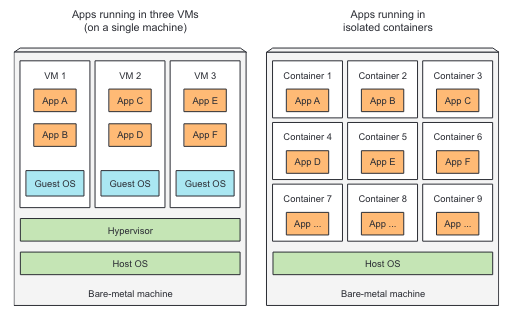
\includegraphics[width=\textwidth]{gfx/chapters/2_grundlagen/container-vs-vm.png}
  \caption{Virtualization vs. Container Technologie}
  \label{fig:container:vergleich}
  \source{\cite{Marko2018}}
\end{figure}

In \ref{fig:container:vergleich} wird der Unterschied von \acp{VM} und Containern dargestellt. 
Jede Anwendung wird innerhalb eines Containers betrieben, sodass eine vollständige Isolation der Prozesse
stattfinden kann \cite{Marko2018}.

Die Isolation von Containern findet mit der Nutzung von \emph{Linux Namespaces} und \emph{Linux Control Groups (cgroups)} statt \cite{Marko2018}.
Namespaces sorgen für die Isolation der Prozesse, 
während cgroups ein Limit für Ressourcen eines Prozesses festlegen können \cite{Marko2018}.

Container ermutigen Entwickler nach dem Konzept \emph{Immutable Infrastructure} zu arbeiten \cite{Burns2019}.
Das Immutable Infrastructure Prinzip besagt, dass sobald eine Version, beziehungsweise ein Artefakt, einer Softwarekomponente erstellt wird,
Nutzer keine Änderungen an diesem Artfakt vornehmen dürfen \cite{Burns2019}. 
Anstatt auf einem Server eine neue Version der Anwendung einzuspielen, werden neue Container Abbilder mit dem erstellen Artefakt gebaut, 
und der laufende Container mit dem neuen Abbild ersetzt \cite{Burns2019}.

\subsection{Docker}
Docker dient als Umgebung zum Verwalten, Erstellen und Betreiben von Containern \cite{Marko2018}.
Dabei besitzt Docker 3 grundliegende Konzepte:

\paragraph{Images}
Images sind Abbilder einer Anwendung und dessen Umgebung.
Es besitzt ein Dateisystem, sowie alle Dateien, die während des Erstellprozesses dem Image hinzugefügt wurden \cite{Marko2018}.

\paragraph{Registries}
Registries sind Speicherorte für Images. Sobald ein neues Image erstellt wird, kann es in eine Registry \emph{gepushed} werden,
um es für andere Systeme zur Verfügung zu stellen \cite{Marko2018}.

\paragraph{Container}
Docker Container sind reguläre Linux Container, die von einem Image erstellt wurden \cite{Marko2018}.
\section{Kubernetes}
\label{sec:grundlagen:kubernetes}
Seit der Einführung von Google in 2014 hat sich Kubernetes zu einer der größten und populärsten 
Open Source Projekte der Welt entwickelt \cite{Burns2019}. Es ist zum Standard für die Entwicklung von cloud-native 
Anwendungen geworden \cite{Burns2019}. 

Kubernetes ist ein System, mit dem eine große Anzahl an Containeranwendungen einfach bereitgestellt und verwaltet werden können \cite{Marko2018}.
Im System werden alle Anwendungen als deklarative Konfigurationsobjekte dargestellt, welche einen gewünschten
Status des Systems abbilden. Kubernetes muss dabei sicherstellen, dass der tatsächliche Status dem gewünschten entspricht \cite{Burns2019}.
Dabei ist es ein \emph{Selbstheilendes System}.
Das bedeutet, das System überwacht den aktuellen Status kontinuierlich, um Abweichungen zu erkennen \cite{Burns2019}.
Als anwendungsorientierte Container-API kann Kubernetes eine Abstraktion von spezifischen \acp{VM} für Entwickler kreieren \cite{Burns2019}.
Entwickler müssen nicht wissen, auf welcher \ac{VM} ihre Anwendung bereitgestellt wird.
Maschinen können somit einfach dem Cluster bei Notwendigkeit hinzugefügt werden \cite{Burns2019}.
\subsection{Architektur}
\label{subsec:kubernetes:architecture}
% TODO: how to cite everything from kubernetes docs?
Die Architektur von Kubernetes besteht aus Rechnern, welche zu einem Cluster zusammengeschlossen werden.
Hierbei besteht das Cluster aus einer oder mehreren \textbf{Worker machines}, welche in Kubernetes \emph{Knoten}
genannt werden. Diese Knoten sind dafür zuständig die eigentliche Last, die \textbf{Pods}, zu betreiben.
Die Kontrollebene\footnote{Containerorchestrationsschicht, welche die API zum Definieren, Bereitstellen und Verwalten von Containern bereitstellt}
ist verantworlich für die Verwaltung von Knoten und Pods innerhalb des Clusters. 
Um Fehlertoleranz und eine hohe Verfügbarkeit zu gewährleisten, besitzt ein Kubernetes Cluster mehrere Knoten und
die Kontrollebene läuft verteilt über mehrere Systeme \cite{kubernetesComponents}. 

\begin{figure}
  \centering
  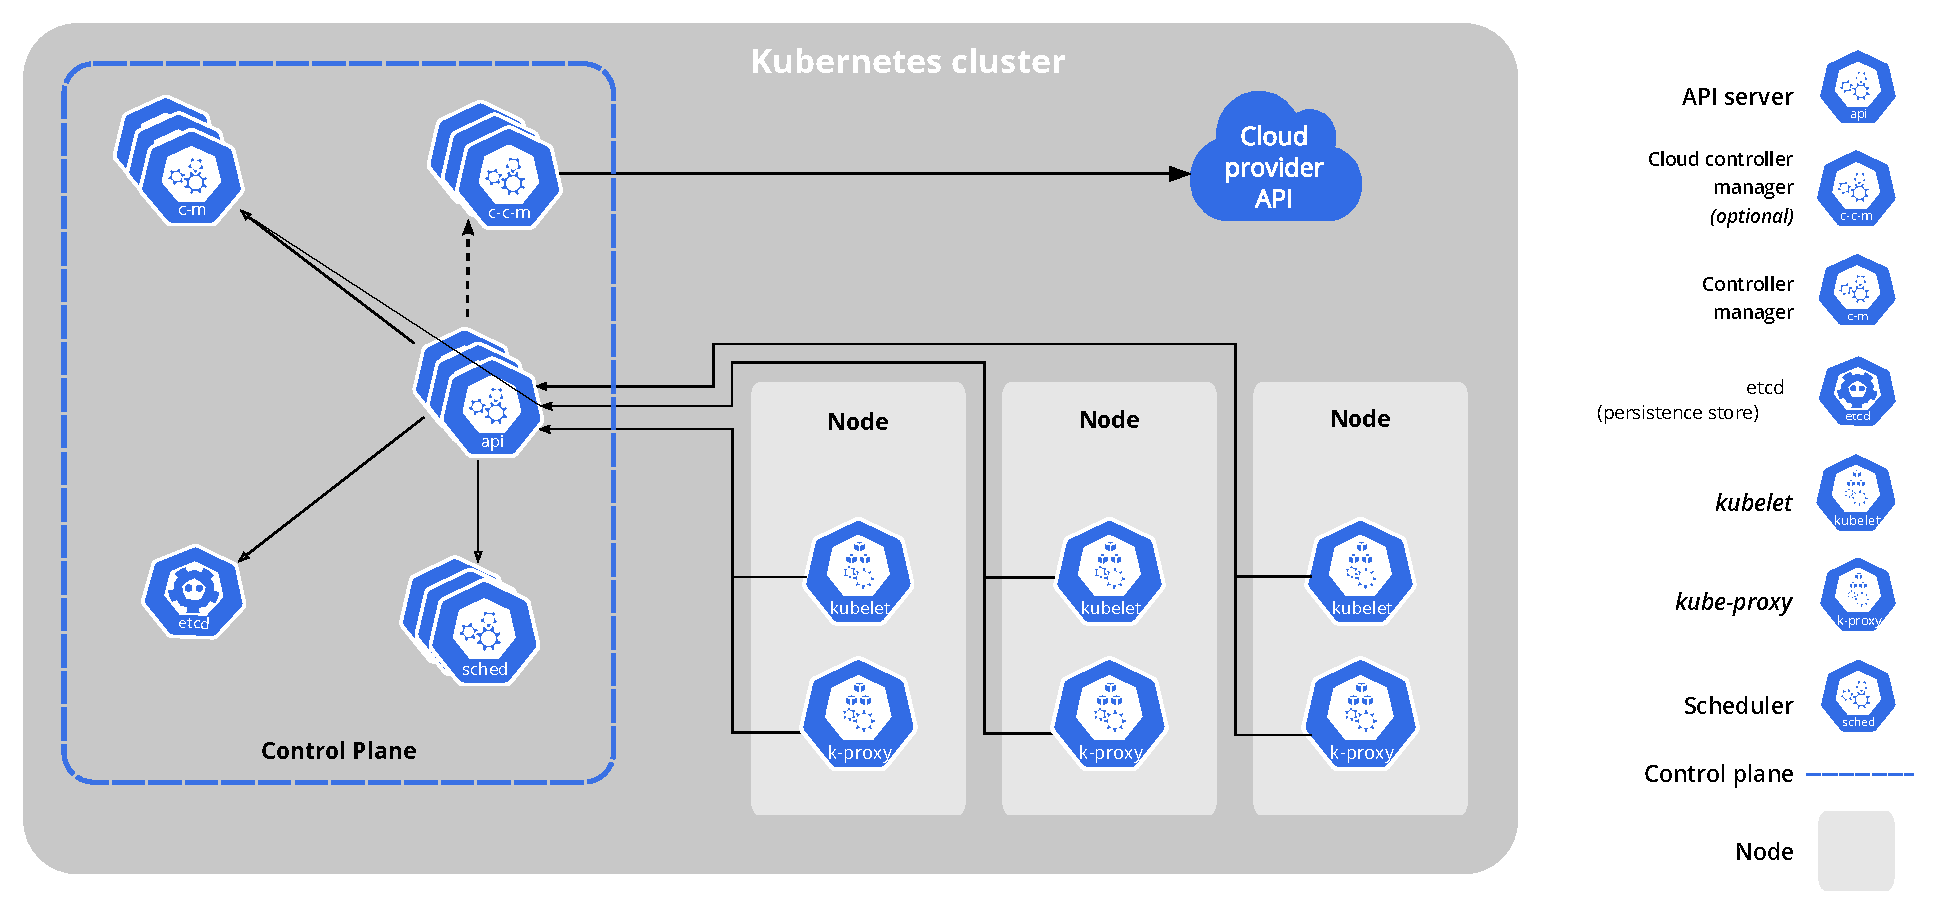
\includegraphics[width=1.2\textwidth]{gfx/chapters/2_grundlagen/components-of-kubernetes.pdf}
  \caption{Architektur eines Kubernetes Clusters}
  \source{\cite{kubernetesComponents}}
  \label{fig:kubernetes_architecture}
\end{figure}

In \ref{fig:kubernetes_architecture} werden die einzelnen Komponenten eines Kubernetes Clusters dargestellt.
Die Kontrollebene besteht dabei aus den folgenden Teilen:
\begin{itemize}
  \item etcd
  \item kube-scheduler
  \item kube-apiserver
  \item kube-controller-manager
\end{itemize}

\paragraph{Etcd} dient als Key-Value Speicher für jegliche Cluster Daten.
Der API-Server ist hierbei die einzige Komponente im Cluster, welche direkt mit dem verteilten Speichersytem interagiert \cite{Hausenblas2019}.

\paragraph{Kube-Scheduler} wird im Cluster eingesetzt, um neu erstellte Pods einem Knoten zuzuweisen.
Hierbei werden Werte wie Ressourcenanforderungen, Hardware, Software oder Richtlinien Beschränkungen 
als Faktoren für die Zuweisung verwendet \cite{kubernetesComponents}.

\paragraph{Kube-apiserver} ist der Einstiegspunkt und die zentrale Managmenteinheit des Cluster \cite{Hausenblas2019}. 
Alle Anfragen an das Cluster werden über den API-Server verarbeitet.
Strukturiert ist der API-Server mithilfe einer REST-HTTP API, welche JSON Daten für Anfragen außerhalb des Clusters
oder Protobuf\footnote{Protobuf ist Googles sprach- und plattformneutraler, erweiterbare Mechanismus zur Serialisierung strukturierter Daten \cite{protobuf}.}
bei der Kommunikation innerhalb des Clusters verwendet \cite{Hausenblas2019}.

\paragraph{Kube-controller-manager} verwaltet Controller innerhalb des Clusters.
Jedem Objekt wird dabei ein eigener Controller zugewiesen.

% TODO: newLine 
\vspace{5mm}
Standardmäßig werden Kontrollebenenkomponenten und Knotenkomponenten auf unterschiedlichen Maschinen ausgeführt,
was nicht zwingend notwendig ist, jedoch zur Hochverfügbarkeit und Ausfallsicherheit beiträgt \cite{kubernetesComponents}. 
Jeder Knoten, der dem Cluster angeschlossen ist, besitzt folgende Komponenten:
\begin{itemize}
  \item Kubelet
  \item Kube-Proxy
  \item Containerlaufzeitumgebung
\end{itemize}

\paragraph{Kubelet} wird als \emph{Agent} auf jedem Knoten im Cluster ausgeführt. 
Es registiert den Knoten am Cluster und ist für die Bereitstellung der Pods zuständig.
Kubelet ist ausschließlich für Container zuständig, die von Kubernetes erstellt wurden \cite{kubernetesComponents}.

\paragraph{Kube-Proxy} ist ein Netzwerk Proxy, der für die Implementierung des Service Konzepts \ref{subsec:kubernetes:service}
zuständig ist. 
Dabei wird sichergestellt, dass die Kommunikation von Pods innerhalb und außerhalb des Clusters möglich ist.

\paragraph{Containerlaufzeitumgebung} betreibt die von Kubelet angeforderten Container für einen Pod. 
Jede Containerlaufzeitumgebung muss das 
\ac{CRI}\footnote{Eine Spezifikation von APIs für Containerlaufzeitumgebungen, um mit Kubelet zu interagieren \cite{cri}.} implementieren.

\subsection{Ressourcen}
\label{subsec:kubernetes:ressourcen}
\section{Gaia-X}
\label{sec:grundlagen:gaia-x}
Europas Plan für digitale Souveränität besteht aus der Cloud- sowie Datenselbstbestimmung.
Cloudsouveränität ist wichtig, um Services zu nutzen, die europäischen Regulierungen entsprechen \cite{Braud2021}.
Gaia-X ist hierfür die Initiative, einen freien Software Stack für Kontrolle, Governance und Erstellung gemeinsamer
Regeln und Richtlinien zu entwickeln \cite{Bonfiglio2021}. 
Dieser Stack soll auf allen bestehenden Cloudtechnologien anwendbar sein, um Transparenz, Souveränität und 
Interoperabilität bei Datenübermittlung und Dienstleistungen zu erreichen \cite{Bonfiglio2021}.

\subsection{Architektur}
\label{subsec:gaia-x:architektur}
\paragraph{Design Prinzipien}
Die Gaia-X Architektur beruht auf den folgenden Design Prinzipien:

\subparagraph{Föderationen}
Föderalisierte Systeme beschreiben autonome Einheiten, die durch eine spezifizierte Reihe von Normen,
Frameworks und Regeln verbunden sind.
Das Prinzip soll mit einer minimalen Anzahl an Vorgaben die Interoperabilität und den Informationsaustausch
zwischen den einzelnen Einheiten der Föderation ermöglichen. 
Dabei soll gleichzeitig das Höchstmaß an Autonomie gewährleistet werden \cite{GaiaXArchitecture2021}.
Durch Föderationen können Serviceanbieter ihre Infrastruktur auf vertrauenswürde Weise miteinander verbinden,
um ein verteiltes Cloud-Modell anzubieten \cite{Bonfiglio2021}.

\subparagraph{Dezentralisierung}
Mitglieder einer Föderation sollen selbstorganisiert, ohne zentrale Kontrolle, operieren.
Das Föderationsprinzip ermöglicht diese Selbstorganisation durch die Bereitstellung eines Netzworks
zur Interaktion mit anderen Gaia-X Teilnehmern \cite{GaiaXArchitecture2021}.

\subparagraph{Offenheit}
Eine offene Architektur ermöglicht das einfache Hinzufügen, Aktualisieren und Änderung von Komponenten, sowie
Einblicke in alle Teile der Architektur und proprietäre Nutzung von Software.
Dadurch ist Gaia-X offen für zukünftige Innovationen und Standards und fortschreitende Technologie \cite{GaiaXArchitecture2021}.

\begin{figure}[h]
  \centering
  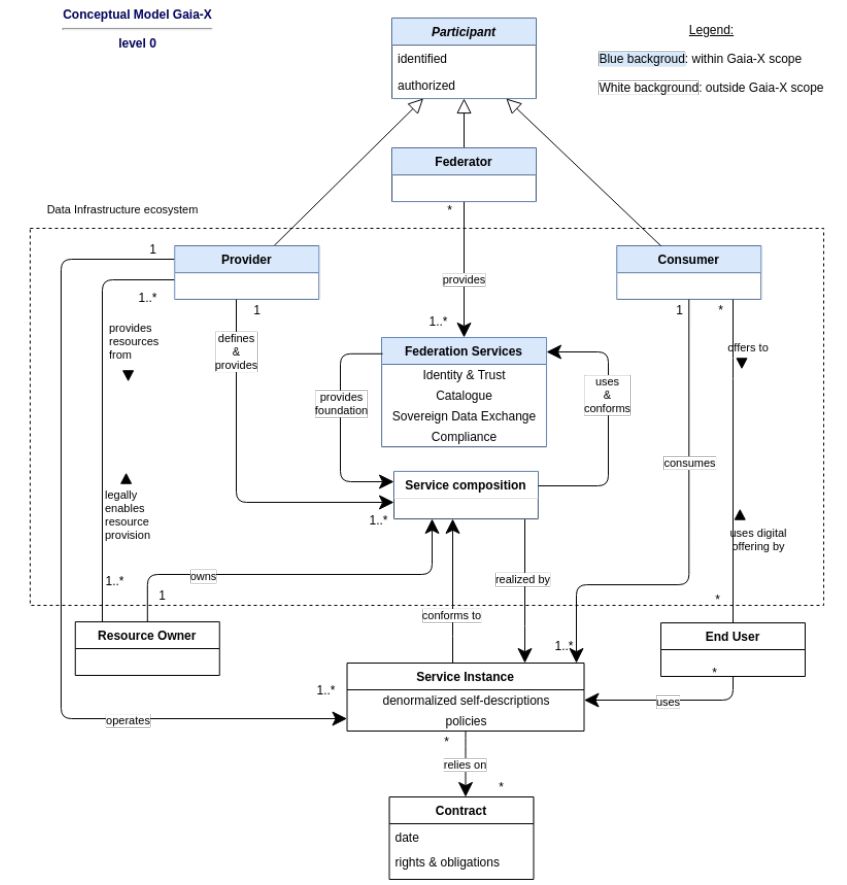
\includegraphics[width=\textwidth]{gfx/chapters/2_grundlagen/gaia-x-architecture.png}
  \caption{Konzeptuelles Modell der Gaia-X Architektur}
  \source{\cite{GaiaXArchitecture2021}}
  \label{fig:gaia-x-concept-architecture}
\end{figure}

\paragraph{Architekturkonzept}
In \ref{fig:gaia-x-concept-architecture} wird das Architekturkonzept, sowie den Umfang von Gaia-X verdeutlich.
Der obere Teil des Modells zeigt die verschiedenen Akteure innerhalb von Gaia-X, während der
untere Teil den Umfang und die Beziehung der Akteuere außerhalb von Gaia-X darstellt.

\subparagraph{Participants}
Participants sind Teilnehmer innerhalb von Gaia-X. 
Dabei können sie eine oder mehrere Rollen einehmen: Föderalist, Anbieter oder Konsument \cite{GaiaXArchitecture2021}.

\subparagraph{Anbieter}
Anbieter sind Teilnehmer, die Ressourcen im Gaia-X Ecosystem bereitstellen. Zudem stellt
ein Anbieter Services mit deren allgemeinen Geschäftsbedingungen und technische Richtlinien bereit \cite{GaiaXArchitecture2021}.

\subparagraph{Föderalist}
Ein Föderalist ist für die Implementierung der Föderationsservices (\ref{subsec:gaia-x:federationservices}) 
sowie für die Koordination der Teilnehmer zuständig \cite{GXFS2021}.

\subparagraph{Konsument}
Konsumenten nutzen Services im Gaia-X Ecosystem um digitale Angebote für Kunden zu ermöglichen \cite{GaiaXArchitecture2021}.

\subsection{Föderationsservices}
\label{subsec:gaia-x:federationservices}
Föderationsservices können als minimale technische Anforderungen zur Operativität der Föderation angesehen werden \cite{GXFS2021}.
Dabei werden Services definiert, welche zur Erfüllung der Ziele von Gaia-X, Vertrauen und Interoperabilität
aufzubauen, sowie die Sicherstellung von Datensouveränität für Teilnehmer zu gewährleisten, beitragen \cite{GXFS2021}.
Zum Start des Gaia-X Projekts werden die folgenden vier Services definiert:

\paragraph{Identität und Vertrauen}
Teilnehmer einer Föderation nutzen diesen Service, um Authentifizierung und Authorisierung innerhalb der Föderation zu nutzen \cite{GXFS2021}.

\paragraph{Föderalisierter Katalog}
Der Katalog dient als zentrales Repository einer Föderation.
Er ermöglicht Teilnehmern das Finden von Informationen und Dienste anderer Föderationsteilnehmer durch Nutzung von
\emph{Self-Descriptions} (\ref{sec:gaia-x-einbettung:gaia-x-katalog}) \cite{GXFS2021}.

\paragraph{Datensouveränität}
Dieser Service hilft Teilnehmer der Föderation Kontrolle und einen Überblick über ihre Daten zu behalten.
Dabei werden Verfahren implementiert, um Transparenz und Kontrolle über Datennutzung zu definieren \cite{GXFS2021}.

\paragraph{Konformität}
Konformitätsservices ermöglichen die Überprüfung der gemeinsamen Services in einer Föderation auf Einhaltung
von Gaia-X Prinzipien wie Datensicherheit \cite{GXFS2021}.

\section{Software as a Service}
\section{Komponenten des Services}
\section{Architektur}
\label{sec:komponenten:architektur}

Die dieser Arbeit zugrunde liegende Architektur folgt dem Ansatz von\cite{Truyen2016}, in dem eine Container basierte
Architektur für \ac{SaaS} Anwendungen vorgestellt wird. Kubernetes spielt hierbei eine wichtige Rolle. Es dient dem State
Managment, der Isolation der Workloads sowie der Authentifizierung für Tenants. Hierbei ist jeder Kontrollservice für den \ac{SaaS}
mit Kubernetes integriert.

\begin{figure}[h]
  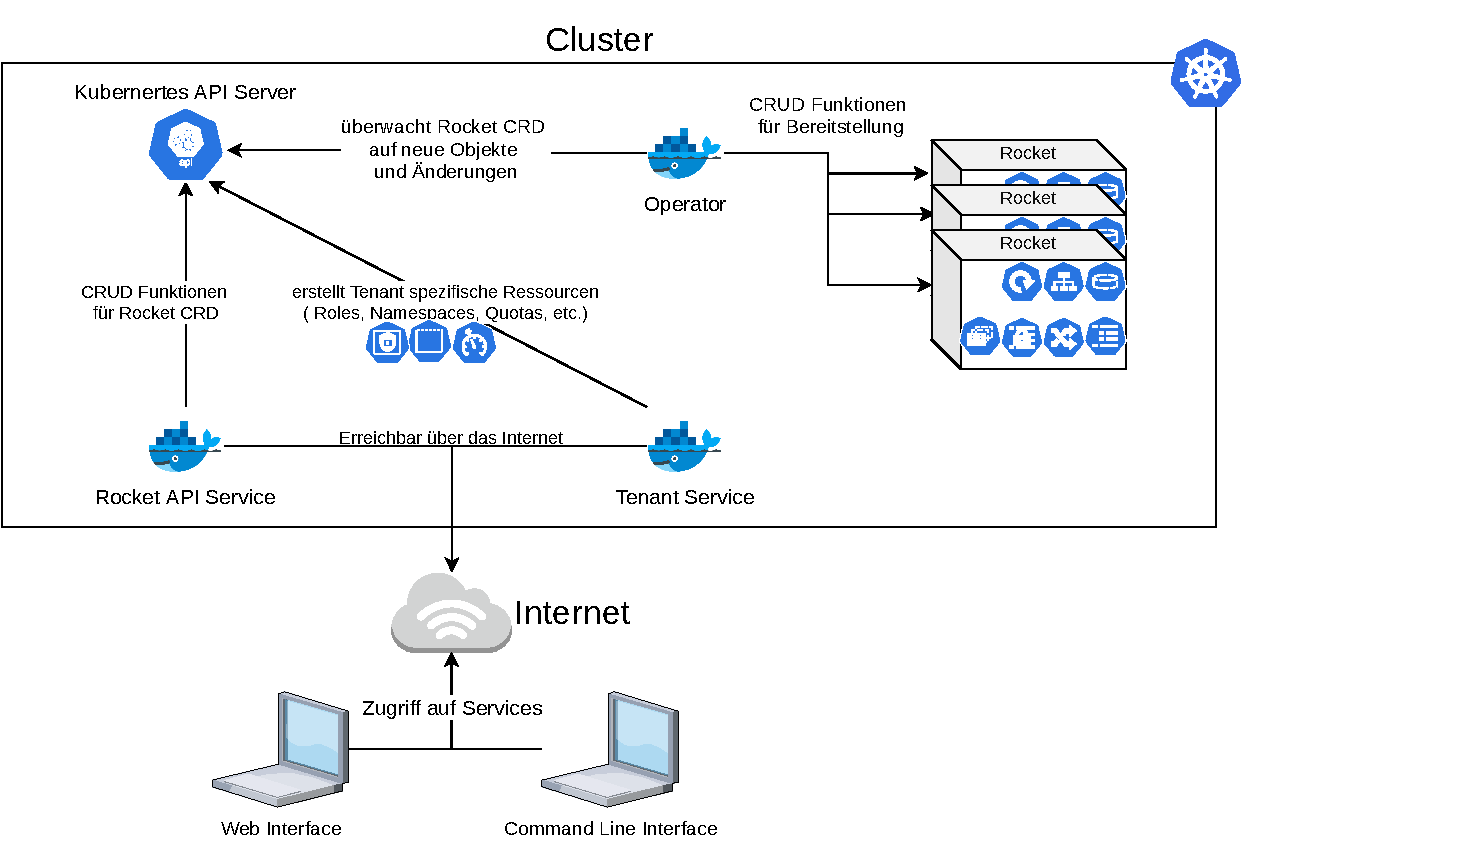
\includegraphics[width=45em]{gfx/chapters/3_komponenten/saas_architecture.pdf}
  \caption{Architektur des \ac{SaaS}}
  \label{fig:architektur}
\end{figure}

In \ref{fig:architektur} wird die Architektur nochmal bildlich dargestellt.
Hier erkennt man, dass die Hauptkomponenten der Serverseite alle mit der Kubernetes API kommunizieren,
um den gewünschten State des Clients zu erzielen. Der Operator \ref{sec:komponenten:operator} dient als Komponente zum tatsächlichen
Erstellen der Rocket und Mongodb Container sowie Netzwerk-, Anwendungs- und Speicherkonfiguration.
Bei einer Änderung der Spezifikation eines Rocket Objekts, wird automatisch eine Synchronisation des 
Clusters vorgenommen, sodass die gewünschte Konfiguration im Cluster deployed ist.
% TODO: Include Ref to CRD Chapter

Der Rocket API Service \ref{sec:komponenten:rocket-api-service} hat die Aufgabe, 
dass vom Operator definierte \ac{CR} im Kubernetes Cluster zu erstellen, während der Tenant Service\ref{sec:komponenten:tenant-service}
sich um die Konfiguration des Users im Cluster kümmert.
Hierbei werden Ressourcen wie bspw. Rollen, Namespaces und Quotas erstellt.

Clients \ref{sec:komponenten:clients} haben die Rolle, mit dem Nutzer zu interagieren. Hierbei kann jegliche Art genutzt werden,
zum Beispiel ein \emph{\ac{CLI}} Tool\footnote{Programm zur Interaktion mit dem User via Kommandozeile}
, \emph{\ac{IaC} Tools} oder ein \emph{Web Interface}. Aus Zeitgründen wurde für die Referenzimplementation nur
ein \ac{CLI} Client implementiert.

\subsection{Operator}
\section{Externe Apps}
\label{sec:komponenten:externe-apps}

Um den Chat Service nun effektiv zu betreiben, werden zusätzliche Open Source Anwendungen zu Nutzen gezogen,
um die Bereitstellung der Rocket Anwendung für den Endnutzer deutlich zu vereinfachen und den Betrieb leichter zu gestalten.
Hierzu werden die folgenden Kubernetes nativen Anwendungen genutzt:
\begin{itemize}
  \item ExternalDNS
  \item Nginx Ingress Controller
  \item Cert-Manager
\end{itemize}

Zudem kommen mit dem Nutzen der Gaia-X Cloud, welche auf OpenStack basiert, der Service \textbf{Designate}
für die DNS Konfiguration und \textbf{Cinder} als Storage Service dazu. 
Designate und die Kubernetes Anwendung \textbf{ExternalDNS} werden miteinander
verwendet, um für neue Ingress Ressourcen automatisch DNS Einträge zu erstellen. 

Der \textbf{Nginx Ingress Controller} dient als Reverse Proxy für alle Ingress Ressourcen innerhalb des Clusters.
Mithilfe des in \ref{sec:komponenten:operator} genannten Synchronisationsmechanismus wird der Nginx Webserver so 
konfiguriert, sodass mittels Host Headern in Anfragen an den Server die jeweils richtige Route zu den Containern hergestellt wird. 
Da der Controller als Proxy dient, muss zudem nur eine externe IP für alle Chat Services genutzt werden, was
zu Kostenersparnissen in der Cloud führt. Die DNS Einträge für alle Chat Instanzen werden durch die Nutzung 
von ExternalDNS auch automatisch an die IP des Loadbalancers für den Nginx Controller angepasst.

Um Zertifikate für HTTPS Verbindungen zu nutzen, wird die von JetStack entwickelte Anwendung Cert-Manager genutzt,
welche die Erstellung von SSL Zertifikaten für Ingress Ressourcen vereinfacht. Hierbei wird eine \emph{Issuer} Ressource
erstellt, welche als Zertizierungsstelle dient.\cite{CertManager2021} Hierbei gibt es mehrere unterstützte Typen, 
wobei für die Referenzimplementation die Entscheidung zunächst auf selbstsignierte Zertifikate gefallen ist.
Eine Umstellung auf ACME\footnote{Automated Certificate Managment Environment},
wie beispielsweise \href{https://letsencrypt.org/de/}{Let's Encrypt}, welche kostenlose SSL Zerifikate anbieten,
ist jederzeit möglich. 
Beim Erstellen einer Ingress Ressource wird die Annotation \texttt{cert-manager.io/issuer} mit dem gewünschten Issuer angehängt,
auf welche die Cert-Manager Anwendung ein Zertifikat am Issuer erstellt. 
Das in der Ingress Ressource referenzierte TLS Secret wird daraufhin vom Cert-Manager für das Zertifikat genutzt.

\subsection{Identität- und Zugriffsmanagement}
Kubernetes besitzt mit dem \ac{RBAC} System eine Möglichkeit innerhalb des Clusters Zugriffsrechte auf Ressourcen
zu verwalten. In dieser Referenzimplementation soll nun ein außerhalb stehender Dienst für das Identitätsmanagment
zuständig sein. Hierbei wurde auf Basis der \ac{SCS} Architektur \emph{Keycloak} als OpenID Connect Provider gewählt.
OpenID Connect ist eine Schicht überhalb des OAuth Frameworks, welches Clients die Möglichkeit bietet, Endnutzer
an einer Authentifizierungsstelle zu verifizieren und Informationen über diese zu erhalten \cite{OpenID2021}.


Kubernetes unterstützt ebenfalls das OpenID Connect Protokoll, indem Optionen für die OpenID Connect Authentifizierungsstelle
übergeben werden. Dadurch ist es für den Endnutzer möglich, sich mittels eines \emph{OpenID Connect Tokens} am 
Kubernetes API Server zu authentifizieren. Die Nutzung dieses Prinzip für den Chat Service wird 
in \ref{sec:komponenten:rocket-api-service} und \ref{sec:komponenten:tenant-service} näher erläutert.
\section{Tenant Service}
\label{sec:komponenten:tenant-service}
Zur Konfiguration des Tenants im Cluster, wurde der Tenant Service zur Verwaltung von Nutzerkonfiguration im Cluster erstellt.
Hierbei wird das gRPC Framework verwendet, um eine konistente API zu ermöglichen. Im Fall des Tenant Service
besitzt die API nur einen \emph{Register} Endpoint. Dieser stellt sicher, dass für den gewünschten Nutzer 
Kubernetes Roles und Rolebindings, ein Cert-Manager Issuer, sowie Resource Quotas angelegt wird. 
Da Rollen an einen Namespace gebunden sind, erhält jeder Tenant einen eigenen Namespace, um sicherzustellen,
dass andere Nutzer keinen Zugriff auf die Ressourcen einer anderen Partei erlangen.
Jene Namespaces werden vom Rocket API Service genutzt, um die entsprechenden Rocket \acp{CR} der Nutzer zu verwalten. 

Im Gegensatz zum Rocket API Service, verwendet der Tenant Service nicht das Prinzip der Identitätsübernahme, da
der Service administrative Bereitstellungen für den Nutzer im Cluster vornimmt. 
Diese Bereitstellung findet mit Hilfe eines Service Accounts, welcher als Identität für Anfragen 
an die Kubernetes API dient, statt . Dieser Service Account besitzt die selben Rechte,
wie die erstellten User Rollen, da Kubernetes nicht erlaubt, Rechte zu vergeben, wenn die anfragende Identität
diese nicht besitzt.


\section{Rocket-API Service}
\label{sec:komponenten:rocket-api-service}
Um Endnutzern nicht die Last von Kubernetes aufzuerlegen, dient der Rocket-API Service als Mittelschicht zwischen
Client und Kubernetes. Hierbei wurde mit Hilfe von Googles gRPC\footnote{\href{https://grpc.io/}{gRPC}} Framework
eine API konzipiert, welche Standard CRUD\footnote{Create, Read, Update, Delete} Operationen, sowie das Auslesen
von Containerlogs implementiert.
Anfragen an die API werden mittels OAuth2 Middleware überprüft, um Authentifizierung zu garantieren. Um sicherzustellen,
dass jeder Nutzer nur auf seine eigenen Services zugreifen kann, werden alle Anfragen an die Kubernetes API als der
Nutzer selbst gestellt. Dies wird durch die Verbindung von Kubernetes, Keycloak und dem Rocket API-Service möglich.
Jeder Client implementiert das OpenID Connect Protokoll, um den Nutzer an der Authentifizierungsstelle, dem Keycloak
Server, anzumelden. Sobald der Client das erhaltene OpenID Token von Keycloak zurück bekommt,
wird es als HTTP Header in jeder Anfrage an den Rocket API-Service mitgeliefert.
Dargestellt ist der beschriebene Ablauf in \ref{fig:rocket-api-service-flow}.

\begin{figure}[h]
  \centering
  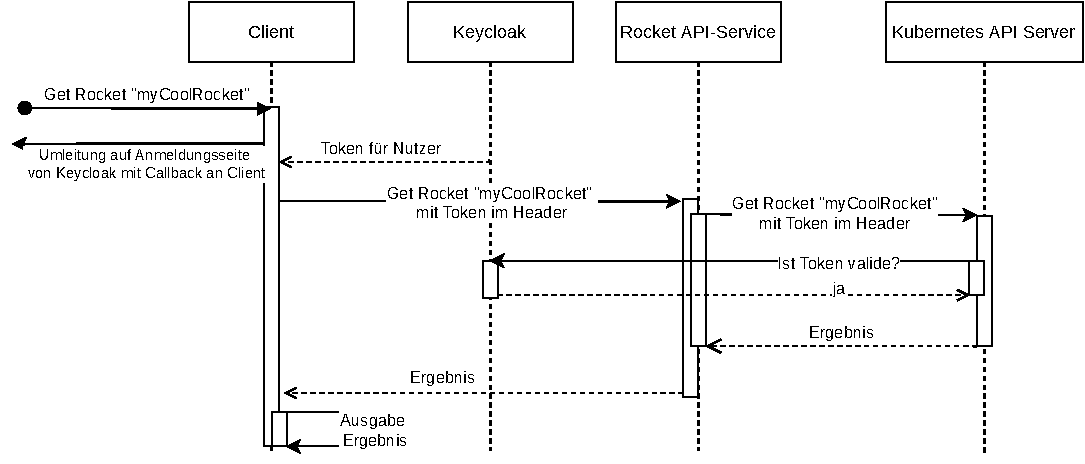
\includegraphics[height=0.5\textwidth]{gfx/chapters/3_komponenten/api-service-flow.pdf}
  \caption{Ablauf des Rocket API-Services}
  \label{fig:rocket-api-service-flow}
\end{figure}

Durch das Auslagern von CRUD Operationen und Tenant Operationen \ref{sec:komponenten:tenant-service} in
verschiedene Services, kann eine unabhängige Entwicklung der beiden Services stattfinden.
\section{Clients}
\label{sec:komponenten:clients}

Clients dienen als Schnittstelle zwischen Endnutzer und den jeweiligen Service APIs. 
\ref{sec:komponenten:tenant-service} \ref{sec:komponenten:rocket-api-service}
Hierfür wurde als Referenzimplementation ein \ac{CLI} Tool erstellt, welches alle API Endpunkte der Services
unterstützt. Zudem besitzt das CLI Tool einen Mechanismus, um OpenID Tokens vom Keycloak Server anzufragen.
Hierbei wird ein minimaler HTTP Server zur Laufzeit erstellt, welcher als \emph{Callback} für den Keycloak Server dient.
Sobald ein Nutzer sich über den Browser in Keycloak anmeldet, wird er auf den Callbackendpunkt des HTTP Servers
zurückgeleitet, welcher das Token persistiert. Dadurch müssen User sich nicht bei jeder Anfrage an die API 
anmelden, sondern die CLI fordert im Hintergrund neue Tokens mit Hilfe des abgelaufenen Tokens an,
um weitere Anfragen zu stellen.
\chapter{Einbettung in Gaia-X kompatible Cloud}
\label{chapter:gaia-x-einbettung}
Gaia-X ermöglicht und fördert die Bildung von Föderationen.
Föderationen dienen als eigenständige Ökosysteme, in denen sich einzelne Teilnehmer zusammenschließen können,
um Services innerhalb oder auch außerhalb der Förderation anzubieten, um Teilnehmern einen Mehrwert zu bieten \cite{GXFS2021}.
Gaia-X operiert nicht, wie alleinstehende Cloud-Providerfirmen, selbst auf dem Markt, sondern erstellt
Software Komponenten zur Erstellung eines föderalisierten Systems in dem mehrere Teilnehmer
untereinander kommunizieren und interagieren können \cite{GXFS2021}.
Als einer der ersten Testimplementationen für Gaia-X gilt die Pluscloud Open,
welche auf Basis des Open Source Projekts \ac{SCS} läuft.
Zum Zweck dieser Arbeit wurde eine zeitlich begrenzte Testlizenz bereitgestellt,
welche die Möglichkeit bietet, die in dieser Arbeit erstellte Referenzimplementation
in einer Gaia-X kompatiblen Umgebung zu testen.


\section{Bereitstellung im Gaia-X Katalog}
\label{sec:gaia-x-einbettung:gaia-x-katalog}
Gaia-X definiert in den Föderationsservices einen Service Katalog, in dem Anbieter Services registrieren
und Konsumenten mittels Suchalgorithmen einen Service für ihre Bedürfnisse finden können \cite{GaiaXArchitecture2021}.
Im Katalog bereitgestellte Services müssen den Nutzer informieren, welche Eigenschaften der jeweilige Service besitzt.
Dadurch können Endnutzer auswählen, welche Services in welchem Standardort 
und zu welchen Umständen, wie die Nutzung des Bereitstellungstools, Betrieb des Service etc. sie nutzen möchten.
Dieses Prinzip wird in Gaia-X \emph{Self-Description} genannt.
Self-Descriptions werden mittels JSON-LD dargestellt, ein
leichtgewichtiges \emph{Linked Data} Format \cite{Eggers2020}.
Betreiber eines Service sind dabei selbst für die Erstellung einer \emph{Self-Description} verantworlich \cite{GaiaXArchitecture2021}.

\begin{figure}
  \centering
  \makebox[\textwidth][c]{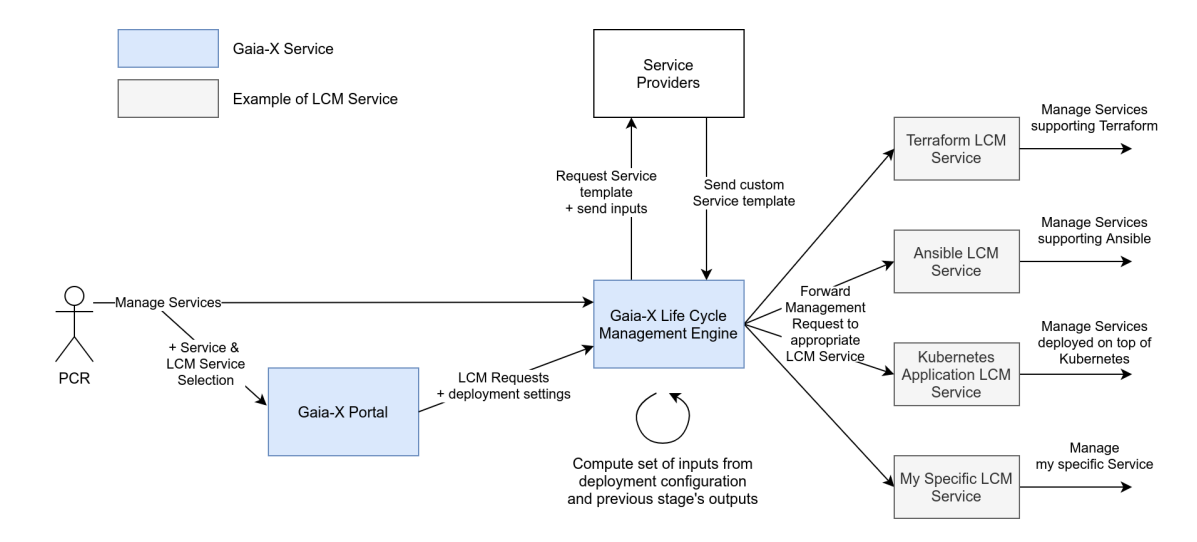
\includegraphics[width=1.35\textwidth]{gfx/chapters/4_gaia-X/orchestration_overview.png}}
  \caption{High Level Übersicht für Gaia-X Service Bereitstellung}
  \source{\cite{ORC2021}}
  \label{fig:gaia-x-orchestration-overview}
\end{figure}

In \ref{fig:gaia-x-orchestration-overview} wird die Kommunikation innerhalb Gaia-X Akteuren
zur Bereitstellung von Services in Gaia-X dargestellt.
Die \ac{LCM} Engine dient als Einstiegspunkt für Kommunikation mit dem Endnutzer. 
Jegliche Verwaltungsanfragen für Services werden an sie gestellt.
 Die Engine verteilt daraufhin diese Anfragen
an den jeweiligen Bereitstellungsservice anhand der Auswahl des Nutzers \cite{ORC2021}.
Im Architekturbild übernimmt die in dieser Arbeit erstellte Referenzimplementation
den Teil des \emph{Kubernetes Application LCM Services}, wobei der \ac{LCM} Service der
Komponente des Rocket API Service entspricht.
Während der Auswahl von Gaia-X Services ist der Nutzer verantwortlich für die Wahl des \ac{LCM} Services \cite{ORC2021}.
Hierbei generiert das Portal eine Liste von möglichen Bereitstellungstechnologien,
weshalb jeder Service in einer \emph{Self-Description} angeben muss, welche Technologien den Service
verwalten sowie bereitstellen (Bereitstellungstechnologien) können \cite{ORC2021}.

Um die Konfiguration eines Services zu gewährleisten, muss der Anbieter eines Services eine Auswahl
an Eingaben, welche erforderlich für die Bereitstellung sind, sowie Standardparameter definieren \cite{ORC2021}.
Im Fall des Rocket Services werden die Eingaben mithilfe der API bereitgestellt.
Der Nutzer des Services muss vor der Nutzung des Services der \ac{LCM} Engine eine Bereitstellungskonfiguration übermitteln.
Diese kann entweder mittels direktem Aufruf an die \ac{LCM} Engine oder dem Gaia-X Portal erstellt werden \cite{ORC2021}.

\begin{figure}[h]
  \centering
  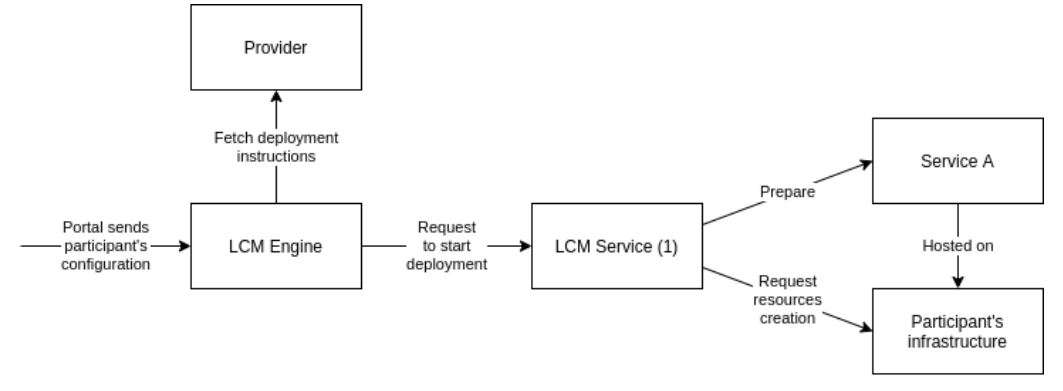
\includegraphics[width=\textwidth]{gfx/chapters/4_gaia-X/example_deployment.png}
  \caption{Beispiel einer Servicebereitstellung}
  \source{\cite{ORC2021}}
  \label{fig:gaia-x-example_deployment}
\end{figure}
Abbildung \ref{fig:gaia-x-example_deployment} verdeutlicht dieses Prinzip anhand eines Beispiels.
Ein Endnutzer übergibt seine gewünschte Konfiguration des Service A via Gaia-X Portal an die \ac{LCM} Engine.
Service A kann dabei allerdings nicht mit allen LCM Services bereitgestellt werden,
sodass der Nutzer sich für den \emph{\ac{LCM} Service (1)} entscheidet.
Die Engine fragt beim Provider nach der Bereitstellungsanweisung für den Service an,
welche nach Zusammenführung mit der Nutzerkonfiguration an den \ac{LCM} Service weitergeleitet wird.
Der \ac{LCM} Service sorgt für die tatsächliche Bereitstellung des Service A
und gibt den Endpunkt des Service an die Engine zurück \cite{ORC2021}.

\section{Sovereign Cloud Stack}
\label{sec:gaia-x-einbettung:scs}

\begin{figure}[h]
  \centering
  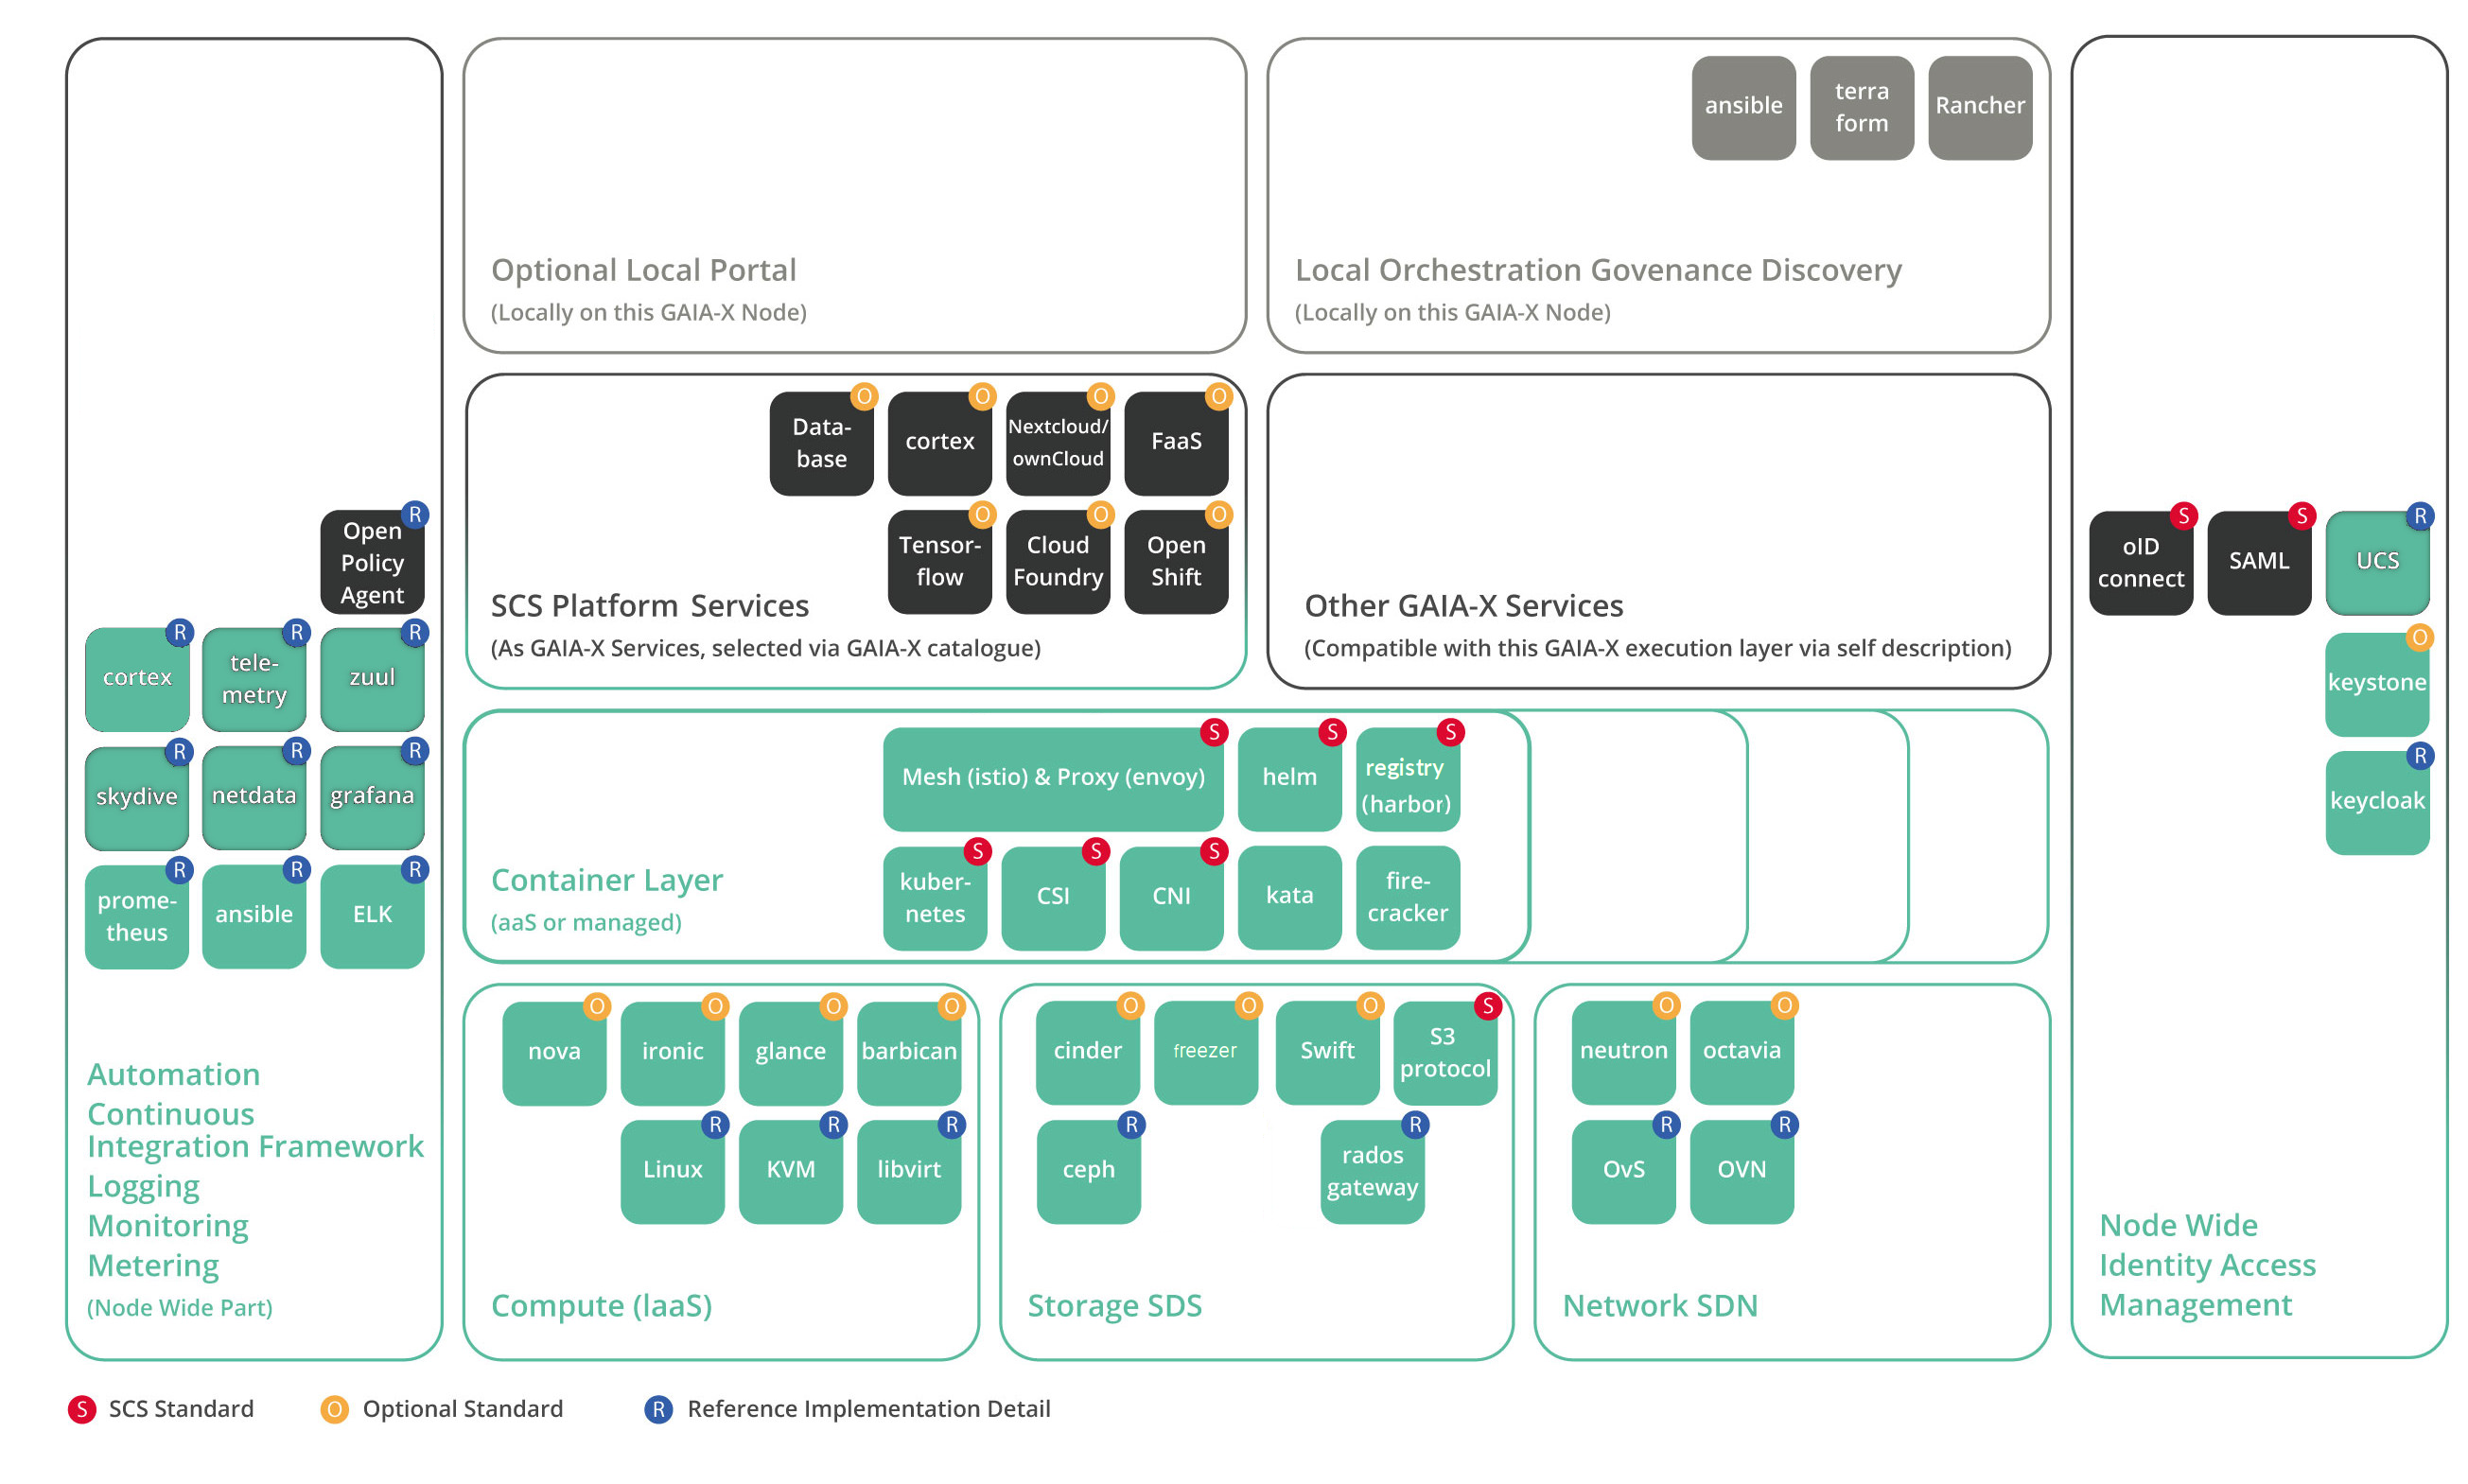
\includegraphics[height=0.71\textwidth]{gfx/chapters/4_gaia-X/scs_architecture.png}
  \caption{Architektur und Komponenten des Sovereign Cloud Stacks}
  \source{https://scs.community/assets/images/201001-SCS-4a.png}
  \label{fig:scs_architecture}
\end{figure}

\ac{SCS} ist ein Open-Source Projekt, um eine standartisierte und souveräne Plattform zu definieren, welche von 
existierenden und zukünfitgen Cloudprovidern genutzt werden soll. 
Ziel des Stacks ist ein Netzwerk von Anbietern, welche durch Nutzung von freier Software und gemeinsamer Standards,
eine interoperable, unabhängige Cloud schaffen \cite{Kagermann2021}.
Als technologischer Standpunkt dient \ref{fig:scs_architecture}, welches die geplante Architektur des \ac{SCS} zeigt. 
Grundlage des Stacks sind OpenStack Services, welche als OpenSource Projekt für Cloud-Computing Architektur entwickelt wurde.
Unterteilt wird dies in 3 grundlegende Bausteine: \textbf{Compute}, \textbf{Network} und \textbf{Storage},
welche als \ac{IaaS} Services definiert sind.
Die Openstack Services sollen als starke, multitenant fähige Basis für Kubernetes Cluster dienen. 
Der Hauptdienst soll Kubernetes as a Service darstellen, auf dem Provider intern ihre \ac{SaaS} aufbauen können \cite{scs}.
Darauf aufbauend wird ein Container Layer erstellt, welcher mit Hilfe von Containerruntimes
wie Docker oder 
Podman\footnote{Daemonlose Containerlaufzeitumgebung zur Verwaltung, Erstellung und Betrieb von Containern \cite{podman}.}
gesteuert werden soll \cite{scs}.

Services wie der in dieser Thesis entwickelte Chat \ac{SaaS} finden sich auf der übergeordneten Ebene \textbf{SCS Platform Services} wieder.
Für die Entwicklung des Rocket Chat \ac{SaaS} wurde diese Architektur als Grundbild genutzt, indem 
genannte Technologien des Stacks in der Implementierung berücksichtigt wurden.
\section{Erstellung der Testinfrastruktur}
\label{sec:gaia-x-einbettung:erstellung-testinfra}
Bei der Erstellung der Testinfrastruktur kam es zu einigen Einschränkungen im Vergleich zu bereits etablierten Hyperscaler Clouds,
da zum Zeitpunkt der Thesis nur Infrastruktur Services wie Netzwerke, DNS, \acp{VM} und Speicher
und kein Managed Kubernetes Service zur Verfügung stehen.
Durch die unterliegende Architektur des Gaia-X Providers kann allerdings bereits etablierte Software
zur Erstellung von Kubernetes Clustern genutzt werden.
Dazu wurde das Tool \textbf{Kubespray}\footnote{\url{https://github.com/kubernetes-sigs/kubespray}} genutzt,
welches mit Hilfe der Konfigurationssoftware \textbf{Ansible} und der \ac{IaC} Software \textbf{Terraform}
\acp{VM}, Netzwerk und Sicherheitsgruppen für die Kubernetes Knoten in der Cloud erstellt.

Aufgrund der zeitlichen Begrenzung der Testlizenz auf 30 Tage wurde jedoch zusätzlich eine lokal
testbare Version der benötigten OpenStack Services erstellt, 
Alle benötigen Services sowie eine vollwertiges Kubernetes Cluster werden in Containern bereitgestellt,
sodass diese lokal betrieben werden können.
Somit kann die Cloudunabhängigkeit von Kubernetes zum Vorteil für Entwickler und der schnellen Entwicklung genutzt werden.
\section{Sovereign Cloud Stack}
\label{sec:gaia-x-einbettung:scs}

\begin{figure}[h]
  \centering
  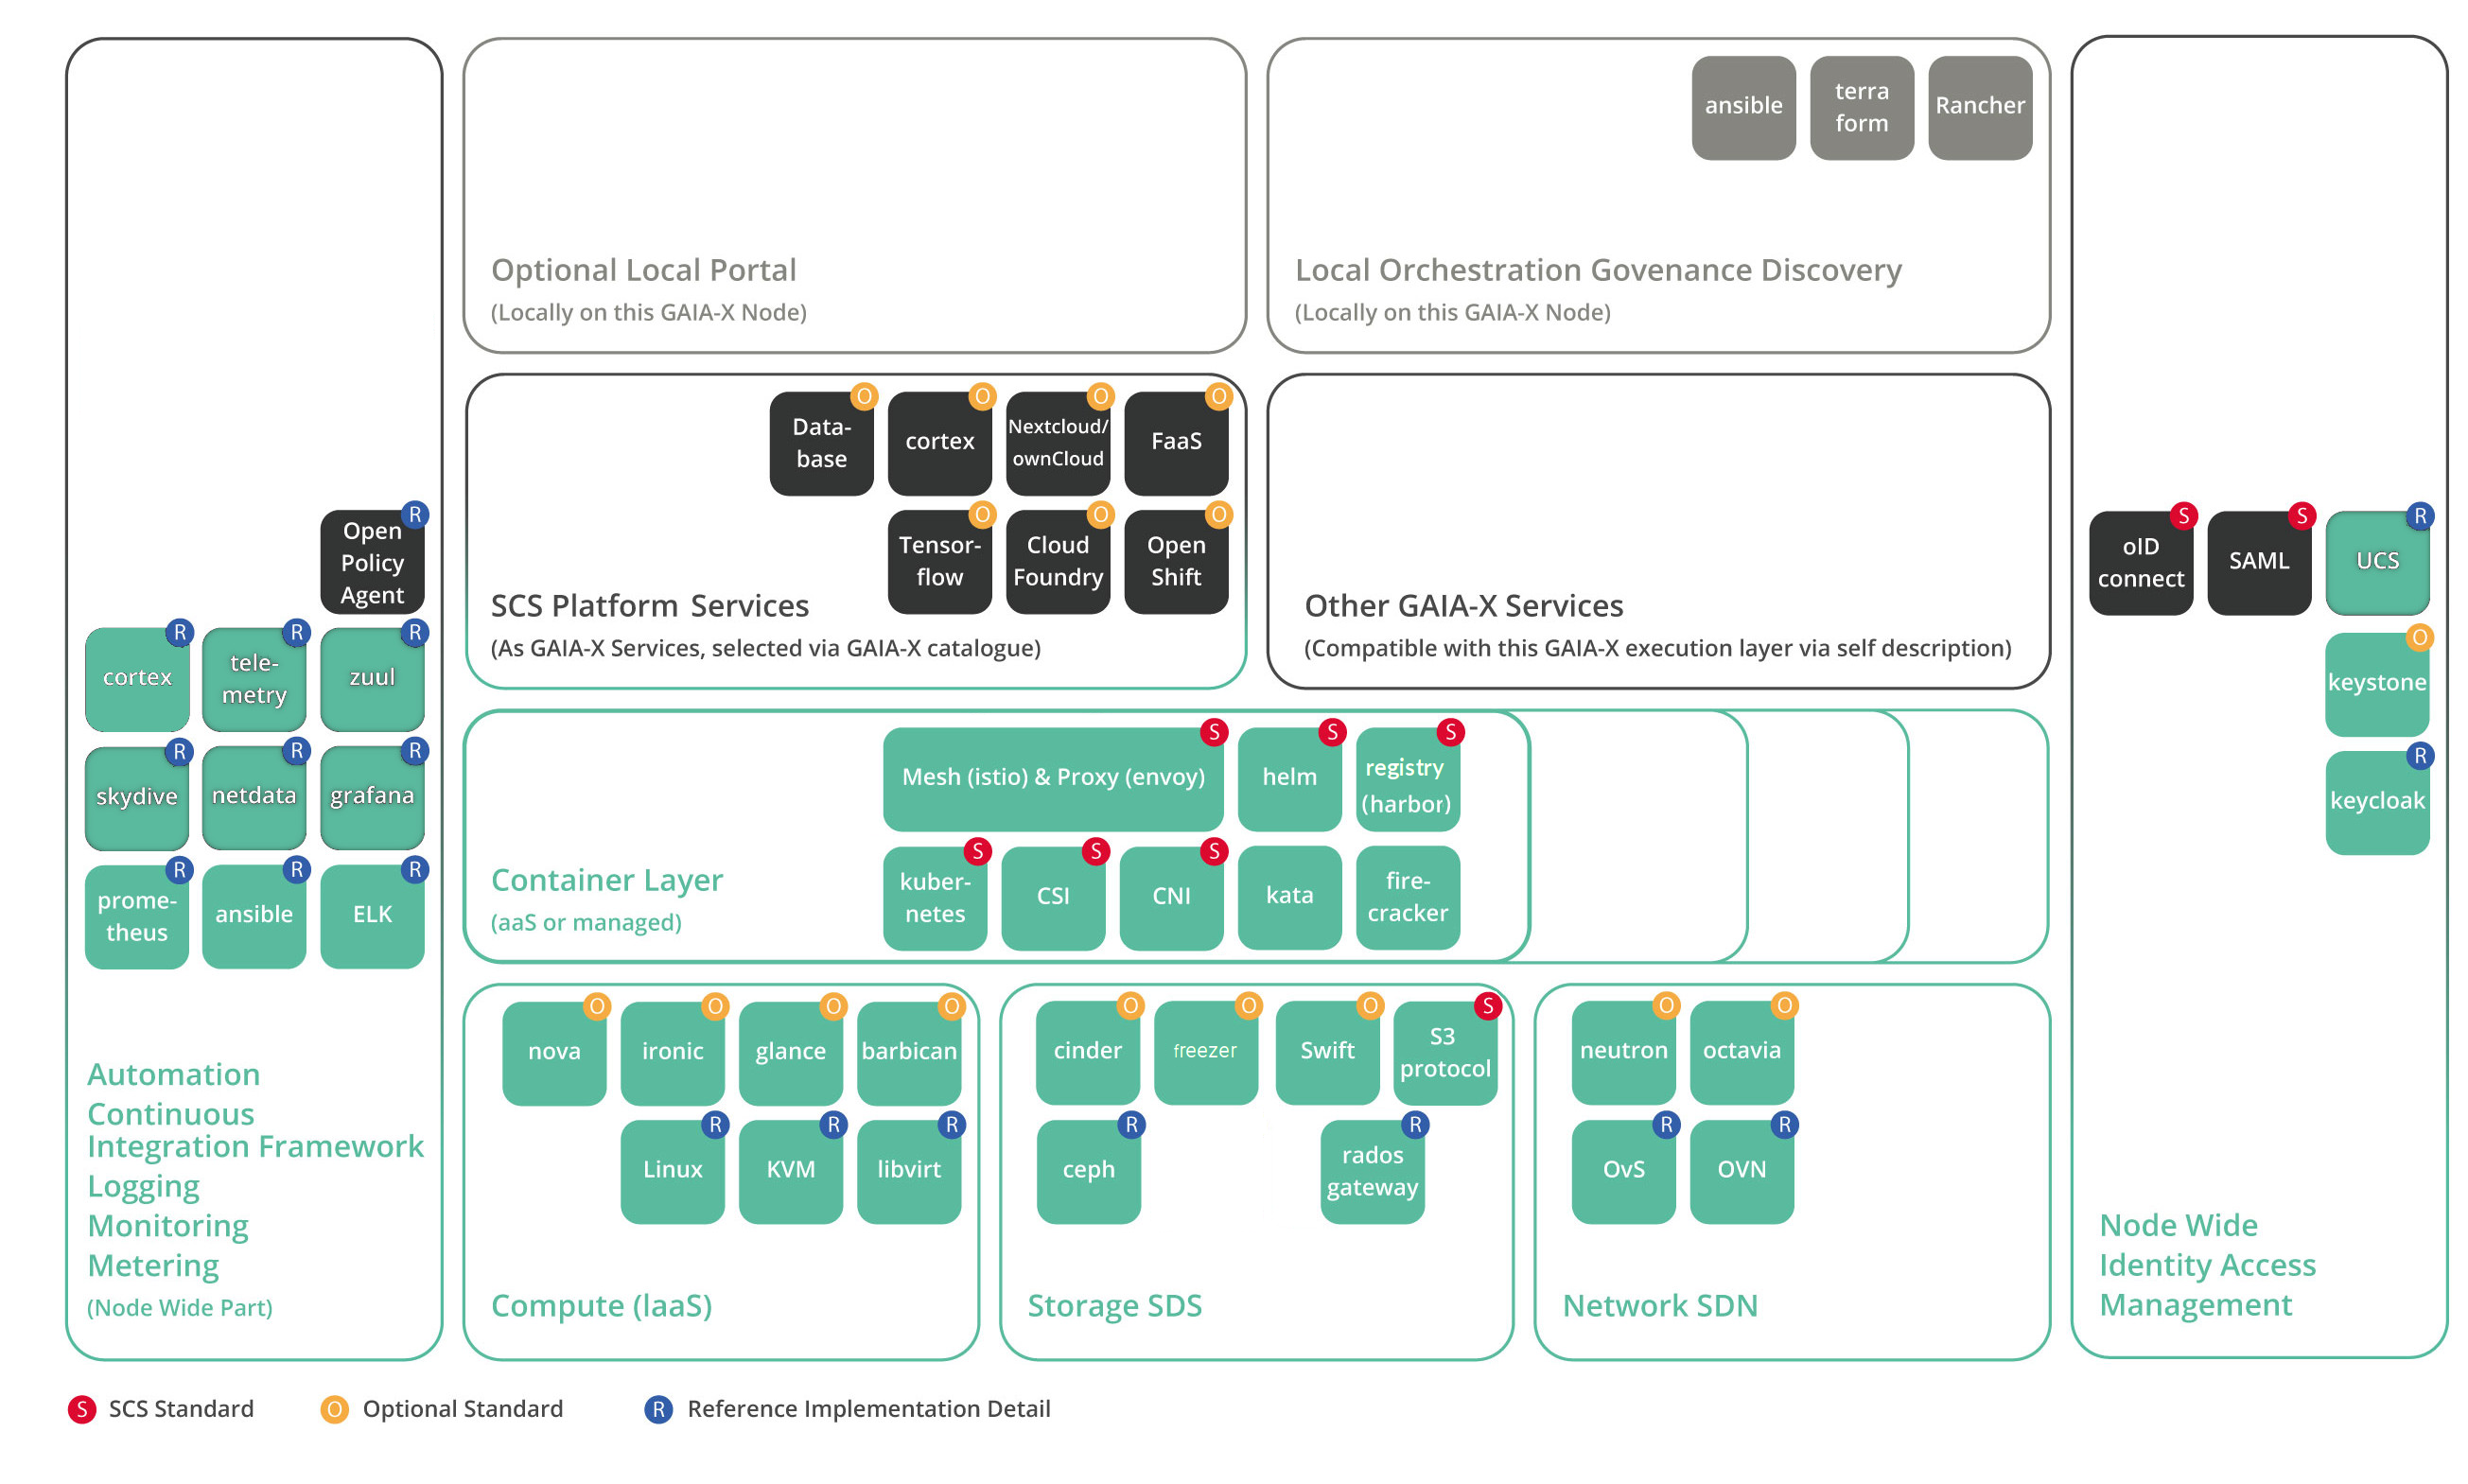
\includegraphics[height=0.71\textwidth]{gfx/chapters/4_gaia-X/scs_architecture.png}
  \caption{Architektur und Komponenten des Sovereign Cloud Stacks}
  \source{https://scs.community/assets/images/201001-SCS-4a.png}
  \label{fig:scs_architecture}
\end{figure}

\ac{SCS} ist ein Open-Source Projekt, um eine standartisierte und souveräne Plattform zu definieren, welche von 
existierenden und zukünfitgen Cloudprovidern genutzt werden soll. 
Ziel des Stacks ist ein Netzwerk von Anbietern, welche durch Nutzung von freier Software und gemeinsamer Standards,
eine interoperable, unabhängige Cloud schaffen \cite{Kagermann2021}.
Als technologischer Standpunkt dient \ref{fig:scs_architecture}, welches die geplante Architektur des \ac{SCS} zeigt. 
Grundlage des Stacks sind OpenStack Services, welche als OpenSource Projekt für Cloud-Computing Architektur entwickelt wurde.
Unterteilt wird dies in 3 grundlegende Bausteine: \textbf{Compute}, \textbf{Network} und \textbf{Storage},
welche als \ac{IaaS} Services definiert sind.
Die Openstack Services sollen als starke, multitenant fähige Basis für Kubernetes Cluster dienen. 
Der Hauptdienst soll Kubernetes as a Service darstellen, auf dem Provider intern ihre \ac{SaaS} aufbauen können \cite{scs}.
Darauf aufbauend wird ein Container Layer erstellt, welcher mit Hilfe von Containerruntimes
wie Docker oder 
Podman\footnote{Daemonlose Containerlaufzeitumgebung zur Verwaltung, Erstellung und Betrieb von Containern \cite{podman}.}
gesteuert werden soll \cite{scs}.

Services wie der in dieser Thesis entwickelte Chat \ac{SaaS} finden sich auf der übergeordneten Ebene \textbf{SCS Platform Services} wieder.
Für die Entwicklung des Rocket Chat \ac{SaaS} wurde diese Architektur als Grundbild genutzt, indem 
genannte Technologien des Stacks in der Implementierung berücksichtigt wurden.
\section{Monitoring}
\label{sec:gaia-x-einbettung:monitoring}
\chapter{Service Level Agreements}
\label{chapter:sla}
Endnutzer von Software sind auf dem Weg zur vermehrten Nutzung von \ac{SaaS} Produkten, wodurch
die Qualität und Verfügbarkeit dieser Services ein wichtiger Aspekt ist. Da allerdings die 
Anforderungen der Nutzer sich unterscheiden und es keinen \emph{One Size fits all} Ansatz gibt,
müssen Anbieter und Nutzer gemeinsame Einigungen bezüglich der Erwartungen an den Service getroffen werden.
Um diese Einigungen einzuhalten, muss der Anbieter die Qualitätsanforderungen der Anwendung überwachen \cite{Ranabahu2009}.
In dieser Referenzimplementation soll auf die Basis Qualitätsanforderungen des Chat Services eingegangen werden,
sowie dessen Monitoring mittels freier Software aus der \ac{SCS} Architektur. 
\section{Datenschutz}
\label{sec:slas:datenschutz}
Hyperscaler Clouds wie \ac{AWS}, Microsoft Azure oder \ac{GCP} unterliegen dem amerikanischen \textbf{US Cloud Act}, welcher
den Datenschutz in Europa gespeicherter Daten gefährdet \cite{Kagermann2021}. Der US Cloud Act besagt hierbei,
dass amerikanische Cloud Provider verpflichtet sind, jeglichen Datenverkehr zu einem Kunden zu speichern und 
US-Behörden Zugriff auf jene Daten zu gewährleisten \cite{CloudAct2018}.
Aufgrund dieses Gesetzes besteht beim Cloud Computing ein grundlegendes Problem 
zur \emph{Integrität und Vertraulichkeit der Datenverarbeitung} \cite{Weichert2010}.

% TODO: Compliance Framework
Gaia-X definiert ein Compliance Framework, welches Regeln für Datenschutz aller Services definiert, an die sich
Anbieter halten müssen \cite{}. 


\subsection{Persistenz von Daten}
\label{subsec:datenschutz:persistenz}
Innerhalb des Kubernetes Clusters werden alle Chatnachrichten innerhalb der vom Operator bereitgestellten
MongoDB gespeichert. Im Kubernetes Cluster sind alle Pods der MongoDB Container mithilfe eines StatefulSets 
erstellt. Zur Persistenz wird das vom StatefulSet verwendet PersistVolume genutzt,
welches als Abstraktion für Speicherimplementierungen für Kubernetes dient.
Als Implementierung dieser Abstraktion wird 
Cinder\footnote{Block Storage Service von OpenStack} CSI\footnote{\href{https://github.com/kubernetes/cloud-provider-openstack/tree/master/pkg/csi/cinder}{Cinder CSI}} genutzt. 
Eine Implementation des \ac{CSI} muss hierbei die folgenden Aktionen unterstützen \cite{container-storage-interface_2021}:
\begin{itemize}
  \item Dynamische Provisionierung sowie Löschen von Volumes
  \item Anhängen oder abtrennen von Volumes an einem Knoten
  \item Einhängen und Aushängen von Volumes an einem Knoten.
  \item Verwaltung von sowohl Block- als auch einhängbarer Volumes
  \item Erstellung und Löschen von Snapshots (Quelle eines Snapshots ist immer ein Volume)
  \item Erstellen eines neuen Volumes von einem Snapshot
\end{itemize}

Sobald im Cluster ein \ac{PVC} erstellt wird, kümmert sich die Anwendung um das Bereitstellen von 
Cinder Volumes innerhalb der Cloud mittels dem Cinder Service von OpenStack \cite{cinderCSI}.
Hierbei werden die Volumes immer in der selben Cloudumgebung wie die Knoten erstellt, wodurch der 
Nutzer des Services sicherstellen kann, dass die Daten des genutztes Chat Services immer in der zuvor 
gewählten Region verwahrt werden.
\section{Verfügbarkeit}
\chapter{Related Work, Fazit und Ausblick}
\label{chapter:fazit}

\section{Related Work}
\label{sec:fazit_ausblick:related_work}

In\cite{Truyen2016} beschreiben \citeauthor{Truyen2016}
das Erstellen von \emph{Multi-Tenant}
\acf{SaaS} mithilfe von Container Orchestrierungssoftware wie Kubernetes.
\acp{SaaS} werden immer häufiger auf skalierbaren Plattformen gehostet, um eine hohe Verfügbarkeit sowie Ausfallsicherheit zu gewährleisten.
Innerhalb ihres Papers gehen sie auf die Vor- und Nachteile des Containeransatzes ein.
Ein klarer Vorteil sei die Möglichkeit des Multi-Cloud Modells, da Kubernetes unabhängig der jeweiligen Cloud Anbieter einsetzbar ist.
und einen Standard implementieren.
Isolationsmöglichkeiten zwischen den \emph{Tenants} habe einen hohen Anspruch für Sicherheit und Datenschutz.
Ein weiterer Problemfall sei der hohe Aufwand zum Managment des Deployments\footnote{Bereitstellung} der Anwendung.
Sie präsentieren eine Referenzarchitektur zum Erstellen von Container basierten Multi-Tenant SaaSs.
Einen fehlenden Standard für Container Images bemängeln sie zum Zeitpunkt ihrer Veröffentlichung.
Als weiteren Verbesserungspunkt stellen \citeauthor{Truyen2016} 3 Möglichkeiten zur Isolation von Tenants vor.
Ein Einsatz des Kubernetes Operator Patterns, welche das Deployment der Anwendung an eine Komponente des \acf{SaaS} übergeben wird,
wurde in diesem Falle nicht beachtet. Das Operator Pattern wurde 2016 von CoreOS vorgestellt, wodurch zum Erscheinungszeitpunkt
des Papers dieses noch nicht vorhanden war.

\paragraph{}
Als weitere Möglichkeit zur Abstraktion von Softwaremanagment für Endnutzer entwickeln \citeauthor{Wieder2012} in ihrem Paper
\cite{Wieder2012} ein System, das die Cloud-Kunden von der Last befreit, zu entscheiden, welche Dienste innerhalb einer Cloud zu verwenden.
Dabei wird speziell auf den Fall von MapReduce Operationen eingegangen. Kunden sollen nur entsprechende Ziele definieren, beispielsweise
die Minimierung der Kosten, eine Berechnung, die in der Cloud ausgeführt werden soll, sowie eine Liste von Cloud Services.
Das System erstellt automatisch die Berechnung und optimiert während der Laufzeit die Anwendung basierend auf externen Zuständen.
Ein Problem liegt hierbei bei der Beschränkung auf kurzweilige Berechnungen, welche keine Grundlagen für \acp{SaaS} bieten.

\paragraph{}
Im Paper \cite{Bousselmi2014} wird das \ac{CPP} für SaaSs beschrieben, welches als Hauptziel die Optimierung der Ressourcennutzung
der Cloudkomponenten sowie die Minimerung der Antwortzeit verfolgt.
Eine gelungene Lösung für das \ac{CPP} solle folgende Anforderungen erfüllen:
\begin{itemize}
  \item \texttt{Platzierungsalgorithmus}
  \item \texttt{Infrastrukturbeschreibung}
  \item \texttt{Provisionierungsalgorithmus}
  \item \texttt{Cloudunabhängig}
\end{itemize}
Desweiteren bieten \citeauthor{Bousselmi2014} eine Übersicht der bereits existierenden Lösungen des \ac{CPP} für \acp{SaaS}.
Allerdings wurden nur das Nutzen von \acf{VM} bedacht, welche Nachteile gegenüber Container besitzen.
Da \acp{VM} zusätzlich Hardware virtualisieren müssen, wodurch Ressourcen eingespart werden können \cite{seo2014performance}.
Außerdem besitzen Container eine bessere Kosteneffizienz sowie Performance im Vergleich zu \acp{VM} \cite{soltesz2007container}.

\section{Fazit}
\label{sec:fazit_ausblick:fazit}

Eine \ac{SaaS} Implementation in einer Gaia-X kompatiblen Cloud ist mit dem aktuellen Stand des Gaia-X Projekts zwar schon 
möglich, bringt allerdings noch einige Unvollständigkeiten mit.
Aufgrund von noch sehr unausgereiften Implementierungen der Gaia-X Services ist der produktive Einsatz eines \ac{SaaS}
Modells noch nicht zu empfehlen. 
Zu viele Services, die die europäische Cloud ausmachen sollen, sind nur als Referenzarchitekturen vorzufinden.
Plusserver Open Cloud, die als erste Implementation von Gaia-X betitelt wird und auf dem \acf{SCS} basiert, 
bietet aktuell weitgehend nur \ac{IaaS} Services an.
Diese Services belaufen sich größtenteils auf schlichte OpenStack Services, 
eine Innovation im Vergleich mit anderen Cloudanbietern bleibt dadurch aus.

Kubernetes stellt sich allerdings als attraktive Plattform zum Bereitstellen, Skalieren und Verwalten von \acf{SaaS} heraus.
Das Operator Framework hilft bei der Erstellung von komplexen Anwendungsbereitstellungen durch traditionelles Softwaredesign.
Eine Zukunft des Containerorchestrierungsframework im Gaia-X Umfeld ist durchaus vorstellbar und wird ebenfalls von \ac{SCS}
angestrebt \cite{scs}.

\newpage
\section{Ausblick}
\label{sec:fazit_ausblick:ausblick}

\begin{figure}[h]
  \centering
  \makebox[\textwidth][c]{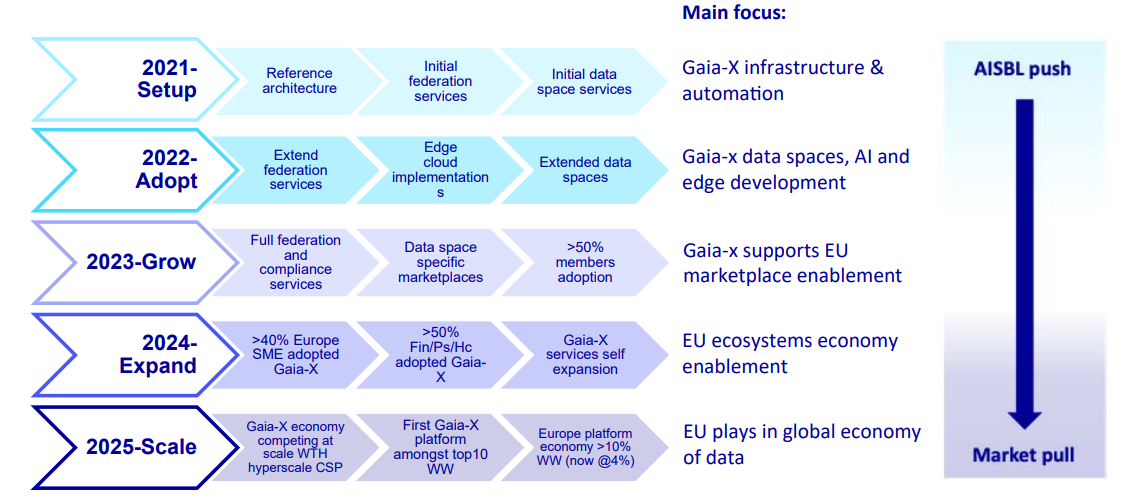
\includegraphics[width=1.3\textwidth]{gfx/chapters/6_fazit_ausblick/gaia-x-ausblick.png}}
  \caption{Fünfjahresplan der Gaia-X Initiative}
  \label{fig:gaia-x-ausblick}
  \source{\cite{Bonfiglio2021}}
\end{figure}

Die Initiative Gaia-X befindet sich zur Zeit noch im Aufbau.
In Abbildung \ref{fig:gaia-x-ausblick} wird der Fünfjahresplan der Initiative dargestellt.
Zum Zeitpunkt der Arbeit läuft die erste Phase: \emph{Setup}.
Eine Implementation der aufgeführten Referenzarchitektur exisitert allerdings noch nicht.

\citeauthor{Bonfiglio2021} strebt im genannten Fünfjahresplan eine vollständige Implementierung der Föderationsservices
im Jahr 2023 an.
Durch die Entstehung eines neuen Markts durch die europäische Cloud soll Gaia-X 2025, in der Phase \emph{Scale},
eine Konkurrenz für Hyperscaler Clouds im globalen Markt werden \cite{Bonfiglio2021}.

\section{Related Work}
\label{sec:fazit_ausblick:related_work}

In\cite{Truyen2016} beschreiben \citeauthor{Truyen2016}
das Erstellen von \emph{Multi-Tenant}
\acf{SaaS} mithilfe von Container Orchestrierungssoftware wie Kubernetes.
\acp{SaaS} werden immer häufiger auf skalierbaren Plattformen gehostet, um eine hohe Verfügbarkeit sowie Ausfallsicherheit zu gewährleisten.
Innerhalb ihres Papers gehen sie auf die Vor- und Nachteile des Containeransatzes ein.
Ein klarer Vorteil sei die Möglichkeit des Multi-Cloud Modells, da Kubernetes unabhängig der jeweiligen Cloud Anbieter einsetzbar ist.
und einen Standard implementieren.
Isolationsmöglichkeiten zwischen den \emph{Tenants} habe einen hohen Anspruch für Sicherheit und Datenschutz.
Ein weiterer Problemfall sei der hohe Aufwand zum Managment des Deployments\footnote{Bereitstellung} der Anwendung.
Sie präsentieren eine Referenzarchitektur zum Erstellen von Container basierten Multi-Tenant SaaSs.
Einen fehlenden Standard für Container Images bemängeln sie zum Zeitpunkt ihrer Veröffentlichung.
Als weiteren Verbesserungspunkt stellen \citeauthor{Truyen2016} 3 Möglichkeiten zur Isolation von Tenants vor.
Ein Einsatz des Kubernetes Operator Patterns, welche das Deployment der Anwendung an eine Komponente des \acf{SaaS} übergeben wird,
wurde in diesem Falle nicht beachtet. Das Operator Pattern wurde 2016 von CoreOS vorgestellt, wodurch zum Erscheinungszeitpunkt
des Papers dieses noch nicht vorhanden war.

\paragraph{}
Als weitere Möglichkeit zur Abstraktion von Softwaremanagment für Endnutzer entwickeln \citeauthor{Wieder2012} in ihrem Paper
\cite{Wieder2012} ein System, das die Cloud-Kunden von der Last befreit, zu entscheiden, welche Dienste innerhalb einer Cloud zu verwenden.
Dabei wird speziell auf den Fall von MapReduce Operationen eingegangen. Kunden sollen nur entsprechende Ziele definieren, beispielsweise
die Minimierung der Kosten, eine Berechnung, die in der Cloud ausgeführt werden soll, sowie eine Liste von Cloud Services.
Das System erstellt automatisch die Berechnung und optimiert während der Laufzeit die Anwendung basierend auf externen Zuständen.
Ein Problem liegt hierbei bei der Beschränkung auf kurzweilige Berechnungen, welche keine Grundlagen für \acp{SaaS} bieten.

\paragraph{}
Im Paper \cite{Bousselmi2014} wird das \ac{CPP} für SaaSs beschrieben, welches als Hauptziel die Optimierung der Ressourcennutzung
der Cloudkomponenten sowie die Minimerung der Antwortzeit verfolgt.
Eine gelungene Lösung für das \ac{CPP} solle folgende Anforderungen erfüllen:
\begin{itemize}
  \item \texttt{Platzierungsalgorithmus}
  \item \texttt{Infrastrukturbeschreibung}
  \item \texttt{Provisionierungsalgorithmus}
  \item \texttt{Cloudunabhängig}
\end{itemize}
Desweiteren bieten \citeauthor{Bousselmi2014} eine Übersicht der bereits existierenden Lösungen des \ac{CPP} für \acp{SaaS}.
Allerdings wurden nur das Nutzen von \acf{VM} bedacht, welche Nachteile gegenüber Container besitzen.
Da \acp{VM} zusätzlich Hardware virtualisieren müssen, wodurch Ressourcen eingespart werden können \cite{seo2014performance}.
Außerdem besitzen Container eine bessere Kosteneffizienz sowie Performance im Vergleich zu \acp{VM} \cite{soltesz2007container}.
\section{Related Work}
\label{sec:fazit_ausblick:related_work}

In\cite{Truyen2016} beschreiben \citeauthor{Truyen2016}
das Erstellen von \emph{Multi-Tenant}
\acf{SaaS} mithilfe von Container Orchestrierungssoftware wie Kubernetes.
\acp{SaaS} werden immer häufiger auf skalierbaren Plattformen gehostet, um eine hohe Verfügbarkeit sowie Ausfallsicherheit zu gewährleisten.
Innerhalb ihres Papers gehen sie auf die Vor- und Nachteile des Containeransatzes ein.
Ein klarer Vorteil sei die Möglichkeit des Multi-Cloud Modells, da Kubernetes unabhängig der jeweiligen Cloud Anbieter einsetzbar ist.
und einen Standard implementieren.
Isolationsmöglichkeiten zwischen den \emph{Tenants} habe einen hohen Anspruch für Sicherheit und Datenschutz.
Ein weiterer Problemfall sei der hohe Aufwand zum Managment des Deployments\footnote{Bereitstellung} der Anwendung.
Sie präsentieren eine Referenzarchitektur zum Erstellen von Container basierten Multi-Tenant SaaSs.
Einen fehlenden Standard für Container Images bemängeln sie zum Zeitpunkt ihrer Veröffentlichung.
Als weiteren Verbesserungspunkt stellen \citeauthor{Truyen2016} 3 Möglichkeiten zur Isolation von Tenants vor.
Ein Einsatz des Kubernetes Operator Patterns, welche das Deployment der Anwendung an eine Komponente des \acf{SaaS} übergeben wird,
wurde in diesem Falle nicht beachtet. Das Operator Pattern wurde 2016 von CoreOS vorgestellt, wodurch zum Erscheinungszeitpunkt
des Papers dieses noch nicht vorhanden war.

\paragraph{}
Als weitere Möglichkeit zur Abstraktion von Softwaremanagment für Endnutzer entwickeln \citeauthor{Wieder2012} in ihrem Paper
\cite{Wieder2012} ein System, das die Cloud-Kunden von der Last befreit, zu entscheiden, welche Dienste innerhalb einer Cloud zu verwenden.
Dabei wird speziell auf den Fall von MapReduce Operationen eingegangen. Kunden sollen nur entsprechende Ziele definieren, beispielsweise
die Minimierung der Kosten, eine Berechnung, die in der Cloud ausgeführt werden soll, sowie eine Liste von Cloud Services.
Das System erstellt automatisch die Berechnung und optimiert während der Laufzeit die Anwendung basierend auf externen Zuständen.
Ein Problem liegt hierbei bei der Beschränkung auf kurzweilige Berechnungen, welche keine Grundlagen für \acp{SaaS} bieten.

\paragraph{}
Im Paper \cite{Bousselmi2014} wird das \ac{CPP} für SaaSs beschrieben, welches als Hauptziel die Optimierung der Ressourcennutzung
der Cloudkomponenten sowie die Minimerung der Antwortzeit verfolgt.
Eine gelungene Lösung für das \ac{CPP} solle folgende Anforderungen erfüllen:
\begin{itemize}
  \item \texttt{Platzierungsalgorithmus}
  \item \texttt{Infrastrukturbeschreibung}
  \item \texttt{Provisionierungsalgorithmus}
  \item \texttt{Cloudunabhängig}
\end{itemize}
Desweiteren bieten \citeauthor{Bousselmi2014} eine Übersicht der bereits existierenden Lösungen des \ac{CPP} für \acp{SaaS}.
Allerdings wurden nur das Nutzen von \acf{VM} bedacht, welche Nachteile gegenüber Container besitzen.
Da \acp{VM} zusätzlich Hardware virtualisieren müssen, wodurch Ressourcen eingespart werden können \cite{seo2014performance}.
Außerdem besitzen Container eine bessere Kosteneffizienz sowie Performance im Vergleich zu \acp{VM} \cite{soltesz2007container}.
\section{Fazit}
\label{sec:fazit_ausblick:fazit}

% TODO: Write
\section{Ausblick}

%*************************************************************************
% Recommendations
%*************************************************************************
%\part{Empfehlungen zur Erstellung wissenschaftlicher Abschlussarbeiten}
%\label{pt:recommendations}
%*************************************************************************
% Backmatter
%*************************************************************************
\appendix
%\renewcommand{\thechapter}{\alph{chapter}}
\cleardoublepage
\part{Appendix}
\chapter{Rocket Custom Resource Spezifikation}
\label{chap:rocketchat_crd_spec}
\lstinputlisting[caption=Rocket CRD Spezifikation]{gfx/chapters/3_komponenten/crd_spec.txt}

%*************************************************************************
% Other Stuff in the Back
%*************************************************************************
\cleardoublepage%********************************************************************
% Bibliography
%*******************************************************
% work-around to have small caps also here in the headline
% https://tex.stackexchange.com/questions/188126/wrong-header-in-bibliography-classicthesis
% Thanks to Enrico Gregorio
\defbibheading{bibintoc}[\bibname]{%
  \phantomsection
  \manualmark
  \markboth{\spacedlowsmallcaps{#1}}{\spacedlowsmallcaps{#1}}%
  \addtocontents{toc}{\protect\vspace{\beforebibskip}}%
  \addcontentsline{toc}{chapter}{\tocEntry{#1}}%
  \chapter*{#1}%
}
\printbibliography[heading=bibintoc]

%*************************************************************************
% Game Over: Restore, Restart, or Quit?
%*************************************************************************
\end{document}
%*************************************************************************
